\documentclass{article}

% Use the unmodified official ICLR 2027 style as soon as it is available in
% ../iclr2027/.  The official Author Guidelines currently link to a ZIP that
% returns HTTP 404 and the ICLR/Master-Template repository has no 2027 files
% as of 2026-08-11.  The fallback keeps this working draft compilable and
% emits a visible build warning; it must not be used for final submission.
\IfFileExists{../iclr2027/iclr2027_conference.sty}{%
  \usepackage{../iclr2027/iclr2027_conference,times}%
}{%
  \usepackage{../iclr2026/iclr2026_conference,times}%
  \PackageWarningNoLine{fcswae}{Official ICLR 2027 style unavailable; using ICLR 2026 preview shell}%
}
\usepackage{graphicx}
\usepackage{booktabs}
\usepackage{placeins}
\usepackage{amsmath,amssymb,amsfonts,amsthm}
\usepackage{xcolor}
\usepackage{hyperref}
\usepackage{url}

\graphicspath{{figures/}}
\setcounter{secnumdepth}{2}

\newtheorem{theorem}{Theorem}
\newtheorem{corollary}{Corollary}
\newtheorem{proposition}{Proposition}

\newcommand{\ours}{F-CS-WAE}
\newcommand{\zc}{z_{\mathrm{c}}}
\newcommand{\zs}{z_{\mathrm{s}}}
\newcommand{\muc}{\mu_{\mathrm{c}}}
\newcommand{\mus}{\mu_{\mathrm{s}}}
\newcommand{\R}{\mathbb{R}}
\newcommand{\MMD}{\mathrm{MMD}}
\newcommand{\KL}{\mathrm{KL}}
\newcommand{\HSIC}{\mathrm{HSIC}}
\newcommand{\Dinter}{\Delta_{\mathrm{inter}}}

\title{Marginal Matching Does Not License Factorized Sampling:\\
Auditing Conditional Style Leakage in Factorized Generative Models}

% Keep the source anonymous as well as the rendered submission.  The ICLR
% style hides authors while \iclrfinalcopy remains commented out.
\author{Anonymous Authors}

% \iclrfinalcopy  % Uncomment only for a camera-ready version.

\begin{document}
\maketitle

\begin{abstract}
Factorized generative models often regularize a style latent $\zs$ toward a
fixed prior using only the aggregate posterior $q(\zs)$, then sample $\zs$
independently of the requested class.  This marginal constraint does not
certify the required conditional invariance $\zs\perp y$.  We place the gap
inside an exact decomposition of the latent mismatch induced by factorized
sampling into global style-prior mismatch, conditional style leakage,
semantic-prior mismatch, and within-class dependence between semantic and
style codes.  We then audit a class-structured WAE on MNIST, Fashion-MNIST,
and CIFAR-10 using a fixed held-out protocol.  Although stochastic style
samples have global $\MMD^2$ between $2.9\!\times\!10^{-4}$ and
$5.7\!\times\!10^{-4}$, a held-out logistic probe recovers the label with
$99.76\%$, $88.29\%$, and $68.62\!\pm\!6.19\%$ accuracy, respectively
(chance: $10\%$); permutation-calibrated HSIC rejects independence for every
checkpoint and latent view ($p=1/201$).  Posterior means and samples give
nearly identical results because the learned style posterior is almost
deterministic, a failure mode we report rather than conceal.  Finally,
independent pixel-space classifiers show that replacing the global style
prior with a post-hoc class-conditional prior raises generated-class accuracy
from $0.102$ to $1.000$ on MNIST and from
$0.132\!\pm\!0.016$ to $0.451\!\pm\!0.063$ on CIFAR-10.  Marginal fit alone
therefore neither verifies the claimed factorization nor validates the
sampler built from it.
\end{abstract}

\section{Introduction}
\label{sec:intro}

Matching an aggregate posterior to a Gaussian is a statement about a
marginal.  Class-invariant style is a statement about conditionals.  These
claims are not interchangeable: $q(\zs)$ can equal $\mathcal N(0,I)$ while
the conditionals $q(\zs\mid y=k)$ remain strongly separated.  Any regularizer
that sees only $q(\zs)$ is blind to how its mass is partitioned by $y$.

The distinction matters because factorized models are sampled differently
from how they are encoded.  During training, a decoder sees semantic and
style codes from the same example.  At generation, a class-conditional
semantic prior is combined with an independently drawn global style code.
If style is class-dependent, the decoder receives recombinations that need
not follow the training joint.  Reconstruction, clustering of $\zc$, and a
global prior statistic can all look strong while this sampling contract
fails.

This phenomenon is related to content leakage studied in earlier
content--style models~\citep{ridgeway2018leakage}; our claim is not that label
information in style was previously unknown.  We instead ask what an
independent factorized sampler must match, which parts aggregate objectives
actually constrain, and how those distinctions should be audited.  The
answer is a four-term latent decomposition together with diagnostics whose
latent view and evaluation split are stated explicitly.

Our empirical case study is \ours{} (Factorized Class-Structured Spherical
Cauchy WAE), a label-guided model with a hyperspherical semantic code and a
Gaussian style code.  We use it to expose a failure mode, not to claim a new
state of the art.  A new held-out audit evaluates both the deterministic
posterior mean $\mus$ and stochastic sample $\zs$.  This distinction is
essential: the theory concerns a random variable, whereas representation
probes and deterministic swaps commonly use its mean.

Our contributions are:
\begin{enumerate}
    \item an exact decomposition of factorized-sampler latent mismatch into
    four non-negative and operationally distinct terms;
    \item a view-specific audit protocol using held-out probes,
    permutation-calibrated dependence tests, and decoder-level generation;
    \item evidence on five checkpoints across three datasets that small
    global style MMD coexists with strong label information in stochastic
    style samples; and
    \item a documented posterior-variance collapse that explains the
    agreement between mean- and sample-based diagnostics and delineates the
    present case study's scope.
\end{enumerate}

\section{Related Work}
\label{sec:related}

\paragraph{Aggregate matching and disentanglement.}
VAEs~\citep{kingma2013autoencoding} penalize a per-example KL, whereas
WAEs~\citep{tolstikhin2017wasserstein} directly match aggregated posteriors
using objectives such as MMD~\citep{gretton2012kernel}.  The averaged VAE KL
decomposes into an information-capacity term and an aggregate-prior
mismatch~\citep{hoffman2016elbo}; neither component alone certifies that a
designated style code is independent of a particular label.  $\beta$-VAE,
$\beta$-TCVAE, FactorVAE, and DIP-VAE penalize capacity, total correlation, or
aggregate moments~\citep{higgins2017beta,chen2018isolating,kim2018disentangling,kumar2018dipvae}.
These constraints differ from $I(\zs;y)$, and unsupervised disentanglement is
not identifiable without assumptions on the model or data
\citep{locatello2019challenging}.

\paragraph{Content--style separation and invariance.}
Split-latent models use grouped observations, labels, paired supervision, or
latent optimization to separate specified and residual variation
\citep{mathieu2016disentangling,bouchacourt2018multilevel,jha2018cycle,ilse2020diva,gabbay2020lord}.
Most directly, \citet{ridgeway2018leakage} probe class information in style
posteriors and introduce leakage filtering for recombination.  Variational
fair autoencoders, gradient reversal, Fader Networks, and information-based
invariance objectives explicitly suppress designated nuisance information
\citep{louizos2015variational,ganin2015unsupervised,lample2017fader,moyer2018invariant}.
Our decomposition clarifies why eliminating $I(\zs;y)$ is necessary but does
not, by itself, make an independent sampler match the encoded joint.

\paragraph{Recombination.}
MUNIT and DRIT explicitly combine content with sampled style
\citep{huang2018munit,lee2018drit}; more recent methods use variance patterns
or invertible merging to obtain content--style structure
\citep{wu2025variance,ma2025scflow}.  These works focus on learning useful
separations.  We focus on auditing the probabilistic claim that permits the
two learned variables to be sampled independently.

\section{Factorized Sampling and Its Mismatch}
\label{sec:theory}

Let $q(y)$ denote the empirical label distribution and let an encoder induce
$q(\zc,\zs\mid y)$.  A factorized class-conditional sampler draws
\begin{equation}
    \zc\sim p(\zc\mid y),\qquad \zs\sim p(\zs),
    \label{eq:sampler}
\end{equation}
independently.  In our case $p(\zs)=\mathcal N(0,I)$.  Many aggregate
objectives constrain only
\begin{equation}
    \mathcal L_{\mathrm{style}}=D\!\left(q(\zs),p(\zs)\right),
    \quad q(\zs)=\mathbb E_{q(y)}q(\zs\mid y).
    \label{eq:global-style}
\end{equation}

\subsection{A marginal cannot certify conditional invariance}

\begin{proposition}[No marginal certificate]
\label{prop:nocert}
Let $\zs\sim\mathcal N(0,I)$ and let $\{A_k\}_{k=1}^K$ be a measurable
partition with $P(\zs\in A_k)=1/K$.  Define $y=k$ iff $\zs\in A_k$.  Then
$q(\zs)=\mathcal N(0,I)$ exactly for every marginal divergence $D$, while
$I(\zs;y)=H(y)=\log K$.
\end{proposition}

The construction is intentionally extremal, but the issue is not restricted
to discontinuous partitions.  For example, let $z\sim\mathcal N(0,1)$ and
$P(y=1\mid z)=\sigma(az)$.  Symmetry gives $P(y=1)=1/2$ and leaves the
marginal of $z$ exactly Gaussian, while
$q(z\mid y=1)=2\phi(z)\sigma(az)$ and
$q(z\mid y=0)=2\phi(z)\sigma(-az)$ are smooth, full-support, and increasingly
distinguishable as $a$ grows.  Thus the logical gap persists under regular
conditional densities.  Proofs are in Appendix~\ref{app:proofs}.

\subsection{The four-term mismatch}

\begin{theorem}[Factorized-sampler latent mismatch]
\label{thm:decomp}
For any $q(y)$, define
\begin{equation}
M_{\mathrm{fact}}:=\mathbb E_{q(y)}\!\left[
\KL\!\left(q(\zc,\zs\mid y)\,\|\,p(\zc\mid y)p(\zs)\right)\right].
\end{equation}
Then
\begin{align}
M_{\mathrm{fact}}={}&
\underbrace{\KL(q(\zs)\|p(\zs))}_{\text{(1) global style-prior mismatch}}
+\underbrace{I_q(\zs;y)}_{\text{(2) conditional style leakage}}\nonumber\\
&+\underbrace{\mathbb E_{q(y)}\KL(q(\zc\mid y)\|p(\zc\mid y))}_{\text{(3) semantic-prior mismatch}}
+\underbrace{I_q(\zc;\zs\mid y)}_{\text{(4) within-class dependence}}.
\label{eq:decomp}
\end{align}
All four terms are non-negative.
\end{theorem}

\begin{corollary}[Exact latent sampling-contract match]
\label{cor:valid}
$M_{\mathrm{fact}}=0$ iff
$q(\zc,\zs\mid y)=p(\zc\mid y)p(\zs)$ for $q(y)$-almost every $y$.
Moreover, for a fixed decoder $g$,
\begin{equation}
\mathbb E_{q(y)}\KL\!\left(g_\#q(\cdot\mid y)\,\|\,
g_\#[p(\zc\mid y)p(\zs)]\right)\le M_{\mathrm{fact}}.
\end{equation}
\end{corollary}

The inequality is one-way.  A non-injective decoder can ignore mismatched
latent directions, so latent equality is not necessary for identical decoded
distributions; nor does equality between posterior-decoded and prior-decoded
outputs establish agreement with real data.  Decoder-level evaluation is
therefore complementary to the decomposition.

Table~\ref{tab:audit-map} summarizes the operational consequence.  The four
terms answer different questions and cannot substitute for one another.  In
particular, a small value for term 1 says nothing about term 2, and removing
term 2 still permits the decoder to exploit within-class dependence captured
by term 4.

\begin{table}[ht]
\caption{The four latent requirements and their finite-sample audit.  The
statistics are proxies for distinct properties, not additive estimates of
$M_{\mathrm{fact}}$.}
\label{tab:audit-map}
\centering
\small
\begin{tabular}{clll}
\toprule
Term & Failure source & Required equality & Audit used here \\
\midrule
1 & Style-prior mismatch & $q(\zs)=p(\zs)$ & global MMD \\
2 & Conditional leakage & $q(\zs\mid y)=q(\zs)$ & probe, HSIC, $\Dinter$ \\
3 & Semantic-prior mismatch & $q(\zc\mid y)=p(\zc\mid y)$ & conditional MMD \\
4 & Within-class coupling & $q(\zc,\zs\mid y)=q(\zc\mid y)q(\zs\mid y)$
& conditional HSIC \\
\bottomrule
\end{tabular}
\end{table}

\section{Audit Protocol and Case Study}
\label{sec:protocol}

\subsection{View-specific diagnostics}

We use stochastic posterior samples for claims about the sampling contract
and means for deterministic representations:
\begin{itemize}
    \item \textbf{Term 1:} unbiased multiscale-RBF
    $\MMD^2(\{\zs^i\},\mathcal N(0,I))$.
    \item \textbf{Term 2:} class-mean separation
    $\Dinter=\binom K2^{-1}\sum_{j<k}\|\bar z_s^{(j)}-\bar z_s^{(k)}\|_2$,
    a held-out probe suite, and a multiscale HSIC permutation test between
    style and label.  We compute each on both $\mus$ and a seeded $\zs$ draw.
    \item \textbf{Term 3:} class-conditional semantic MMD is part of training;
    we do not treat a minibatch training loss as a calibrated held-out
    estimate of the KL term.
    \item \textbf{Term 4:} classwise conditional HSIC on $(\muc,\mus)$ with
    within-class permutations.  This is explicitly a mean-view diagnostic,
    not an estimate of conditional mutual information.
\end{itemize}
No finite-sample proxy is presented as an estimate of
$M_{\mathrm{fact}}$ itself.

The fixed audit uses 2,048 test examples and a stratified 60/20/20
probe-train/validation/test split.  Feature standardization is fit on probe
training data only.  We report logistic regression, a fixed two-layer MLP,
RBF-SVM, and $k$-NN; hyperparameters and per-seed values are in
Appendix~\ref{app:protocol}.  HSIC uses 1,024 examples and 200 plus-one
calibrated permutations, so its smallest attainable $p$-value is $1/201$.

\subsection{Case-study model}

\ours{} uses a shared modified ResNet-18 encoder, a hyperspherical semantic
code $\zc\in\mathbb S^{63}$, a Gaussian style code $\zs\in\R^{128}$, and a
residual upsampling decoder.  The encoder trunk feeds separate heads for the
semantic direction and concentration $(\muc,\rho_c)$ and style parameters
$(\mus,\log\sigma_s^2)$.  A forward pass samples both codes and decodes their
concatenation.  Class-specific Spherical Cauchy priors with EMA-updated centers
shape $\zc$; global MMD matches sampled $\zs$ to $\mathcal N(0,I)$.

The complete objective is
\begin{align}
\mathcal L={}&\mathcal L_{\mathrm{rec}}
+\alpha(t)\mathcal L_{\mathrm{class}}
+\beta(t)\mathcal L_{\mathrm{agg}}
+\gamma(t)\mathcal L_{\mathrm{style}}\nonumber\\
&+\delta(t)\mathcal L_{\mathrm{style-cls}}
+\eta(t)\mathcal L_{\mathrm{cls}}.
\label{eq:objective}
\end{align}
$\mathcal L_{\mathrm{rec}}$ combines L1 and LPIPS; the supervised class MMD
matches $q(\zc\mid y=k)$ to its class prior, aggregate semantic MMD matches
$q(\zc)$ to the prior mixture, global style MMD implements
Eq.~\ref{eq:global-style}, and an auxiliary classifier on $\muc$ prevents
semantic collapse.  Training lasts 300 epochs in four phases: reconstruction
warm-up, style regularization and classification, partial semantic matching,
and the full objective.  All coefficients and phase boundaries are listed in
Appendix~\ref{app:model}.

The optional per-class loss
\begin{equation}
\mathcal L_{\mathrm{style-cls}}=
\frac1K\sum_k\MMD^2(q(\zs\mid y=k),\mathcal N(0,I))
\label{eq:perclass}
\end{equation}
targets term 2 but not term 4.  It reuses labels already consumed by the
semantic objective and is therefore a supervised intervention, not a generic
unsupervised disentanglement loss.  The held-out Stage-0 audit below focuses
on unrepaired $\delta=0$ checkpoints to isolate the failure of marginal
matching.  We subsequently use existing $\delta>0$ checkpoints only to test
whether explicitly conditional regularization moves the conditional
distribution statistics in the predicted direction.

\section{Experiments}
\label{sec:experiments}

\subsection{Datasets, checkpoints, and evaluation}

We use MNIST~\citep{lecun1998gradient}, Fashion-MNIST
\citep{xiao2017fashion}, and CIFAR-10~\citep{krizhevsky2009learning}.  MNIST
and Fashion-MNIST remain at their native $28\times28$ resolution; CIFAR-10
remains $32\times32$.  We use the standard train/test splits, scale pixels to
$[0,1]$, and apply no augmentation to the generative models.  Stage-0 uses
MNIST and Fashion-MNIST model seed 0 and CIFAR-10 seeds 0, 1, 2.  All reported
uncertainties are sample standard deviations over model seeds, not probe
reruns.  Each held-out probe test partition contains 410 examples.

We evaluate at three levels.  Latent diagnostics use the fixed protocol of
Section~\ref{sec:protocol}.  Reconstruction uses SSIM and LPIPS
\citep{zhang2018unreasonable}; clustering runs $K$-means on $\muc$ and reports
Hungarian-matched ACC and NMI.  Generation uses FID
\citep{heusel2017gans} and generated-class accuracy (Gen-ACC).  The latter is
scored directly from generated pixels by classifiers trained only on real
data: a four-layer CNN for MNIST (99.34\% real-test accuracy) and a
WideResNet-28-10 for CIFAR-10 (96.16\%)~\citep{zagoruyko2016wide}.  These
classifiers never participate in \ours{} training.

\subsection{The case study is not representation-degenerate}

Our audit would be uninformative if the case-study model failed to encode
classes or reconstruct images at all.  Table~\ref{tab:competence} gives a
sanity check on CIFAR-10.  \ours{} reaches
$0.812\pm0.005$ clustering ACC and $0.655\pm0.008$ NMI across three seeds.
The comparison rows share a modified ResNet-18 and total latent dimension 192
but are single-seed and not equally tuned; we use them only to establish that
the audited representation is nontrivial, not to claim controlled
superiority.

\begin{table}[ht]
\caption{CIFAR-10 competence check.  \ours{} is mean $\pm$ sample standard
deviation over three seeds; reference autoencoders are single-seed.  Lower
FID is better.}
\label{tab:competence}
\centering
\small
\begin{tabular}{lrrr}
\toprule
Method & ACC & NMI & FID \\
\midrule
\ours{} & $.812\pm.005$ & $.655\pm.008$ & $81.9\pm1.5$ \\
AE + cross entropy & .665 & .611 & 144.3 \\
AE + supervised contrastive & .541 & .599 & 275.5 \\
AE + triplet loss & .506 & .502 & 281.4 \\
ResNet autoencoder & .220 & .102 & 121.0 \\
\bottomrule
\end{tabular}
\end{table}
\FloatBarrier

\subsection{Small global MMD coexists with label leakage}

\begin{table}[ht]
\caption{Held-out audit of unrepaired $\delta=0$ checkpoints.  MMD and
$\Dinter$ use stochastic $\zs$; LP columns are test accuracy.  CIFAR-10 is
mean $\pm$ sample standard deviation over three model seeds; the other rows
are single checkpoints.  Chance LP is $10\%$.}
\label{tab:stage0}
\centering
\small
\begin{tabular}{lrrrrr}
\toprule
Dataset & MMD$^2$ & $\Dinter$ & Logit $\mus$ & Logit $\zs$ & RBF $\zs$ \\
\midrule
MNIST & .000572 & 6.264 & 99.76 & 99.76 & 99.76 \\
Fashion-MNIST & .000287 & 4.791 & 88.29 & 88.29 & 93.17 \\
CIFAR-10 & $.000306\!\pm\!.000054$ & $3.954\!\pm\!.269$ &
$68.46\!\pm\!6.29$ & $68.62\!\pm\!6.19$ & $70.16\!\pm\!3.36$ \\
\bottomrule
\end{tabular}
\end{table}

Table~\ref{tab:stage0} gives the central result.  Global MMD is small on all
five checkpoints, yet every held-out probe is far above chance.  Multiscale
HSIC independently rejects $\zs\perp y$ for both $\mus$ and $\zs$ at every
checkpoint ($p=0.00498$).  The result is not specific to linear separation:
the MLP and RBF-SVM reach $90.73\%$ and $93.17\%$ on Fashion-MNIST, and
$70.57\!\pm\!3.50\%$ and $70.16\!\pm\!3.36\%$ on stochastic CIFAR-10 codes.
Full probe results appear in Appendix~\ref{app:full-results}.

The distinction between mean and sample matters conceptually but barely
changes these checkpoints empirically.  Across the reported probe suite the
largest mean--sample difference is $0.49$ percentage points on
Fashion-MNIST and $0.73$ points on any CIFAR-10 seed.  Therefore the leakage
persists in the stochastic variable used by Theorem~\ref{thm:decomp}; it is
not an artifact of probing only $\mus$.
\FloatBarrier

\subsection{Why means and samples agree: posterior-variance collapse}

The style encoder uses
$\zs=\mus+\exp(\tfrac12\log\sigma_s^2)\epsilon$ with
$\epsilon\sim\mathcal N(0,I)$ and clamps log variance to $[-10,10]$.
Direct checkpoint inspection finds $99.9966\%$ of MNIST, $99.9989\%$ of
Fashion-MNIST, and $100\%$ of CIFAR-10 log-variance coordinates at or below
$-10$ before the effective clamp.  Hence the typical posterior standard
deviation is $e^{-5}=0.006738$, tiny relative to between-class separation
$3.95$--$6.26$.  The learned stochastic encoder is thus almost deterministic.

This observation narrows, rather than inflates, our claim.  It explains why
sample-based verification agrees with mean-based diagnostics for these
models, but does not imply that the two views are interchangeable in other
models.  It also exposes a limitation of the aggregate diversity penalty:
class-dependent posterior means can create large batch variance without
maintaining per-example posterior entropy.

\subsection{Conditional distributions reveal what the marginal hides}

The probe result is mirrored by a direct two-sample comparison.  For each
class we compute unbiased multiscale
$\MMD^2(q(\zs\mid y=k),\mathcal N(0,I))$ on the same 2,048-example subset and
average over classes.  Table~\ref{tab:conditional-mmd} compares that value
with the global MMD on seed-0 checkpoints.  With only global style matching,
mean conditional MMD is $21.0\times$ the global value on MNIST and
$15.3\times$ on CIFAR-10.  This is the distributional form of the same
failure: mixture components remain class-specific even when their aggregate
is close to the prior.

\begin{table}[ht]
\caption{Global versus mean per-class style MMD on stochastic $\zs$,
single-seed checkpoints.  The $\delta=1$ model adds
Eq.~\ref{eq:perclass}.}
\label{tab:conditional-mmd}
\centering
\small
\begin{tabular}{llrrrr}
\toprule
Dataset & $\delta$ & Global MMD & Cond. MMD & Ratio & $\Dinter$ \\
\midrule
MNIST & 0 & .000885 & .018600 & 21.01 & 6.212 \\
MNIST & 1 & .001088 & .004763 & 4.38 & 1.222 \\
CIFAR-10 & 0 & .000558 & .008537 & 15.29 & 3.744 \\
CIFAR-10 & 1 & .000675 & .003606 & 5.34 & 1.049 \\
\bottomrule
\end{tabular}
\end{table}

Figure~\ref{fig:conditional-mmd-bars} resolves the class average into its ten
components.  Every class-conditional MMD lies above the dashed global value
on both datasets, so the gap is not driven by one or two exceptional classes.
The marginal statistic is small precisely because it measures the mixture,
not because its class-conditioned components individually match the prior.

\begin{figure}[t]
\centering
\begin{minipage}{0.49\textwidth}
\centering
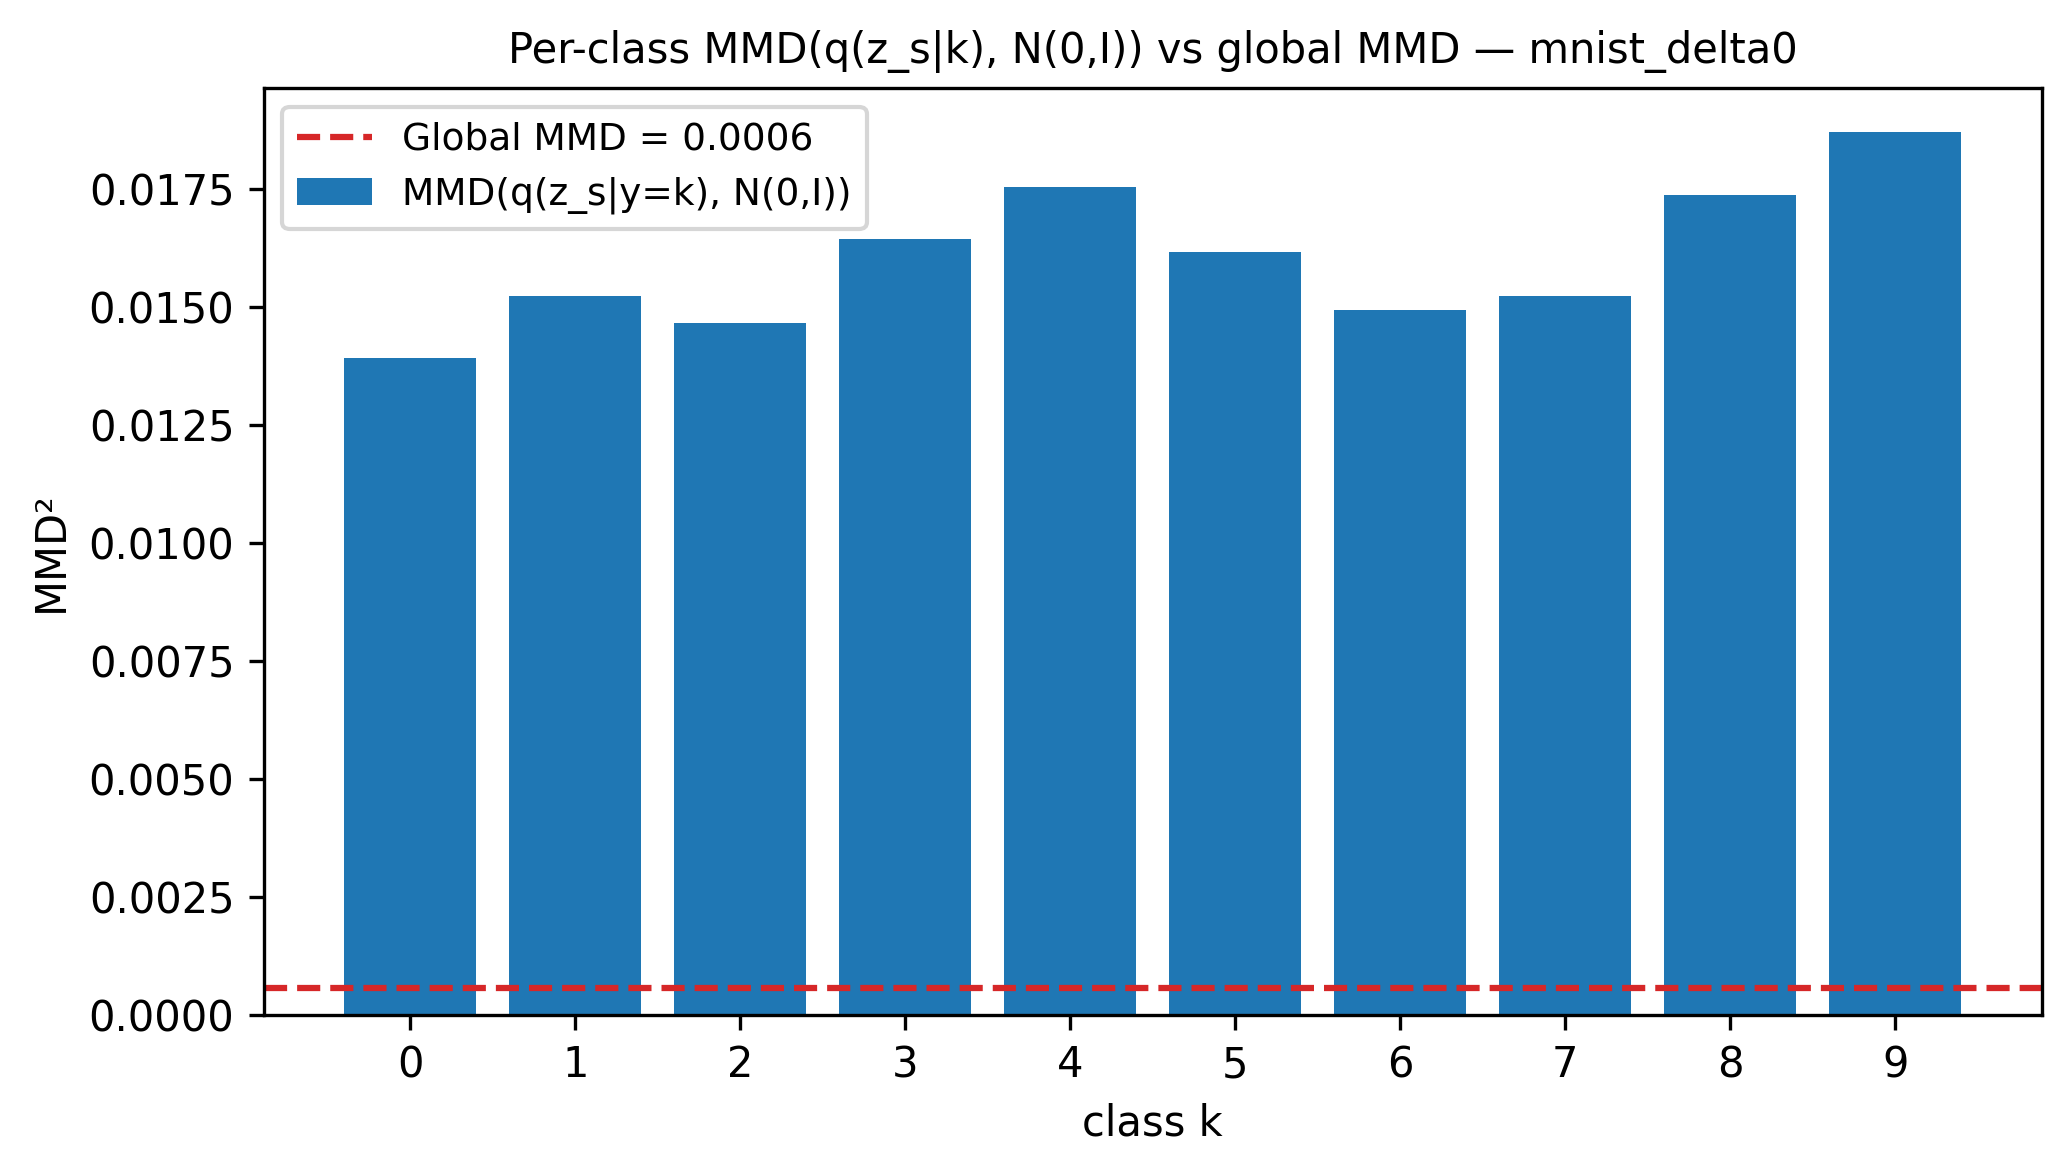
\includegraphics[width=\linewidth,trim=0 0 0 85,clip]{conditional_mmd_per_class_bar_mnist.png}\\[-0.5em]
\small (a) MNIST
\end{minipage}\hfill
\begin{minipage}{0.49\textwidth}
\centering
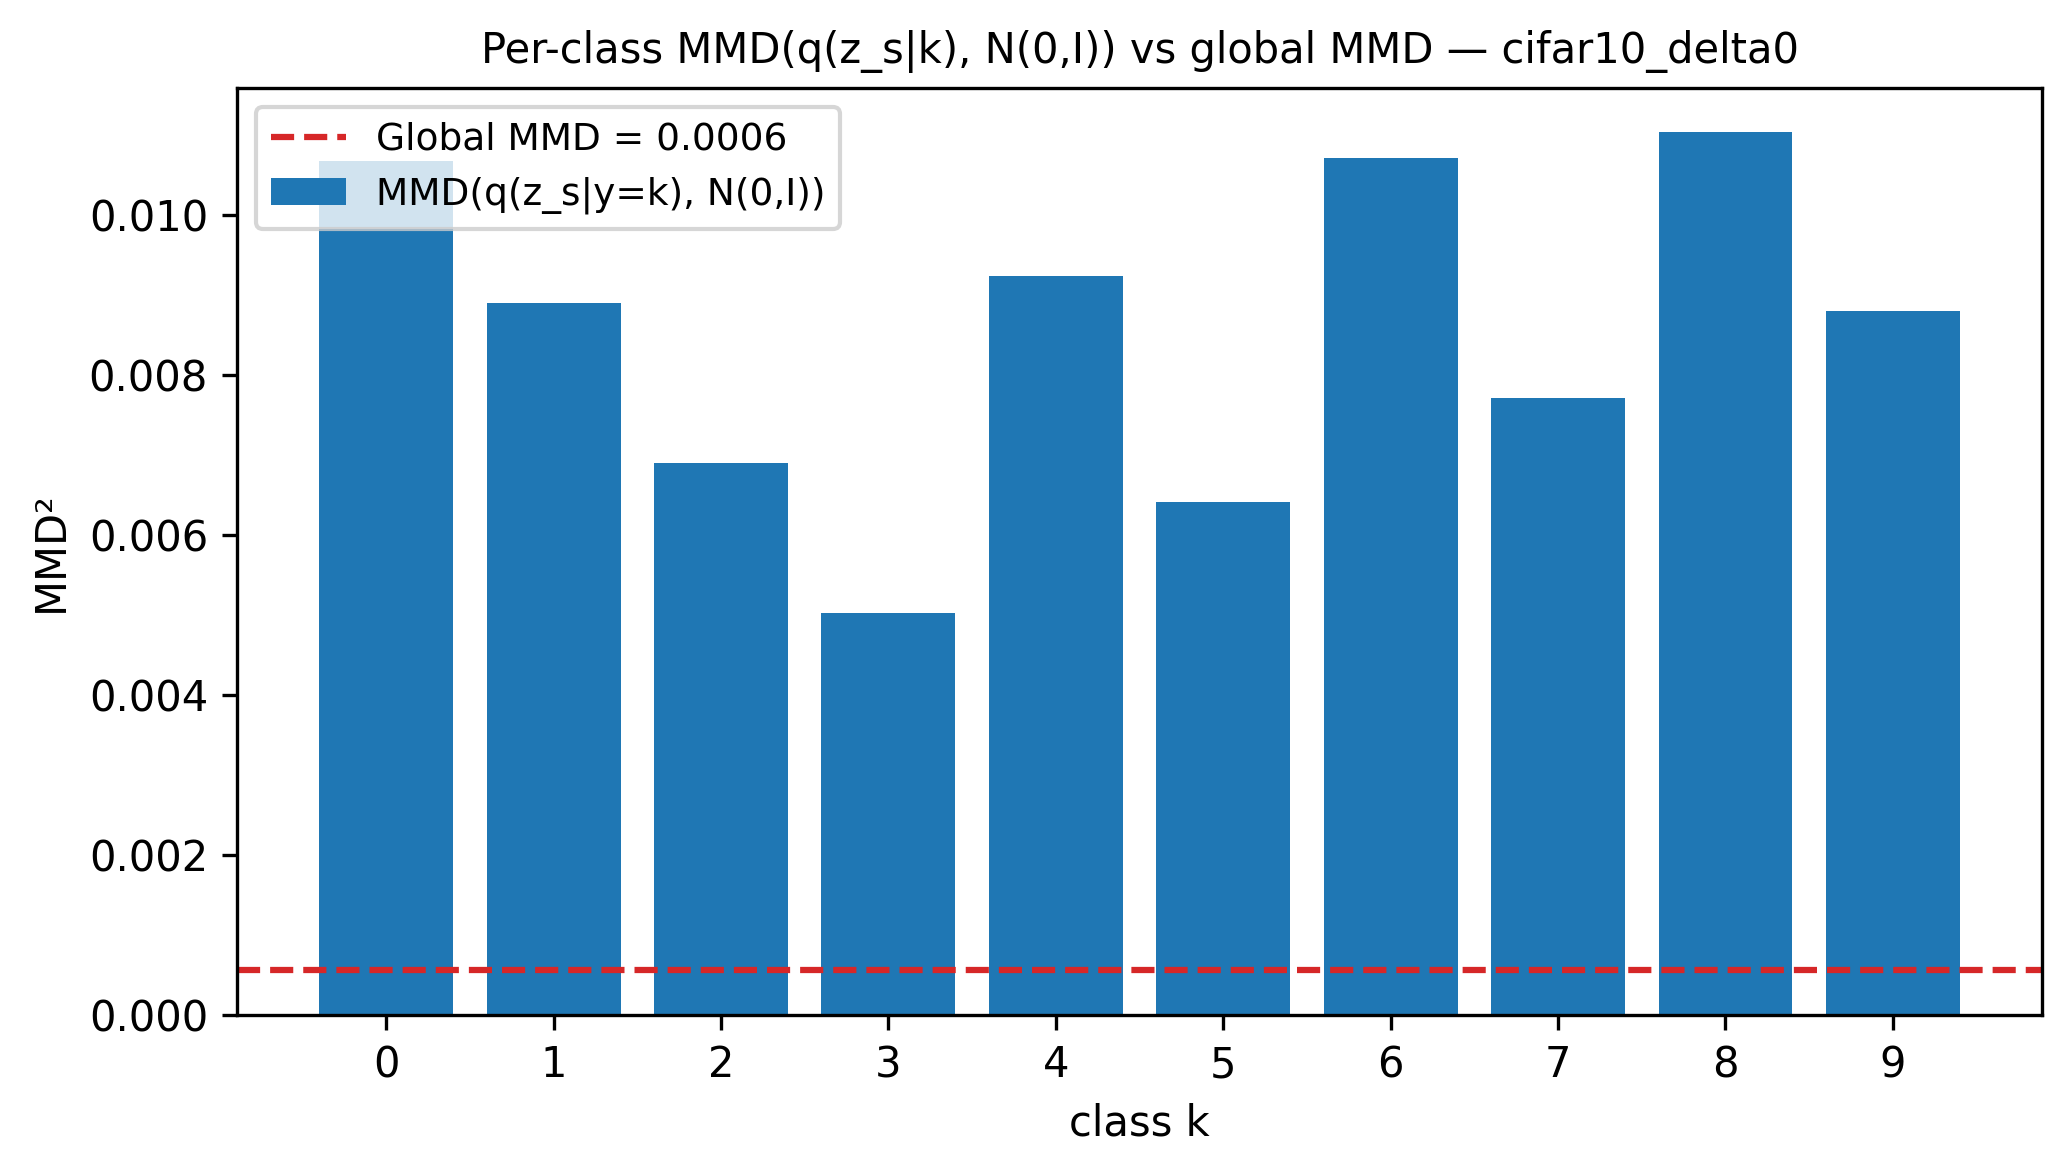
\includegraphics[width=\linewidth,trim=0 0 0 85,clip]{conditional_mmd_per_class_bar_cifar10.png}\\[-0.5em]
\small (b) CIFAR-10
\end{minipage}
\caption{Per-class $\MMD^2(q(\zs\mid y=k),\mathcal N(0,I))$ at
$\delta=0$ on stochastic posterior samples.  The dashed line is the global
$\MMD^2(q(\zs),\mathcal N(0,I))$ optimized by the marginal regularizer.
All ten conditional values exceed it on each dataset.}
\label{fig:conditional-mmd-bars}
\end{figure}

The per-class objective acts in the predicted direction: it reduces mean
conditional MMD by $74\%$ on MNIST and $58\%$ on CIFAR-10, and reduces
$\Dinter$ by $80\%$ and $72\%$, respectively.  It does not make either
conditional statistic vanish, and the global MMD changes little.  We do not
reuse the historical remedy probe accuracy here because those checkpoints
have not yet been regenerated with the held-out Stage-0 probe protocol.

The decomposition also predicts a distinct within-class failure.  On the
unrepaired Stage-0 checkpoints, classwise conditional HSIC between
$(\muc,\mus)$ rejects conditional independence for MNIST, Fashion-MNIST, and
all three CIFAR-10 seeds ($p=1/201$).  The statistics are 0.002440, 0.002459,
and $0.002086\pm0.000222$, respectively.  These are mean-view kernel
statistics rather than estimates of $I(\zc;\zs\mid y)$, but they demonstrate
why successful control of term 2 would not complete the sampling audit.
\FloatBarrier

\subsection{Conditional regularization has a non-monotone trade-off}

Table~\ref{tab:delta-sweep} shows four points from the six-value $\delta$
sweep.  Conditional separation decreases steadily, but clustering and FID
are not monotone.  On MNIST, the $\delta=1$ checkpoint has an isolated ACC
drop that disappears at $\delta=3$; on CIFAR-10, ACC drops at
$\delta=0.3$ and only partially recovers.  Because every sweep point is a
single training seed, these irregularities may be optimization noise and are
not evidence of a causal optimum.

\begin{table}[ht]
\caption{Selected points from the single-seed per-class-MMD sweep.  No
uncertainty or significance claim is made across settings.}
\label{tab:delta-sweep}
\centering
\small
\begin{tabular}{crrr|rrr}
\toprule
& \multicolumn{3}{c}{MNIST} & \multicolumn{3}{c}{CIFAR-10} \\
$\delta$ & ACC & $\Dinter$ & FID & ACC & $\Dinter$ & FID \\
\midrule
0   & .992 & 6.21 & 74.0 & .813 & 3.74 & 80.5 \\
.1  & .990 & 2.12 & 52.6 & .810 & 2.03 & 77.5 \\
1   & .859 & 1.22 & 43.4 & .800 & 1.05 & 74.4 \\
3   & .993 & 1.18 & 41.5 & .799 & .95  & 76.1 \\
\bottomrule
\end{tabular}
\end{table}

Figure~\ref{fig:delta-fid} makes the non-monotonicity visible across all six
archived settings.  The sweep supports a limited conclusion: conditional regularization
consistently compresses class separation in style space, but reduced leakage
does not guarantee monotonic improvement in semantic clustering or image
quality.  It also illustrates why the four terms of
Theorem~\ref{thm:decomp} should be monitored separately.

\begin{figure}[t]
\centering
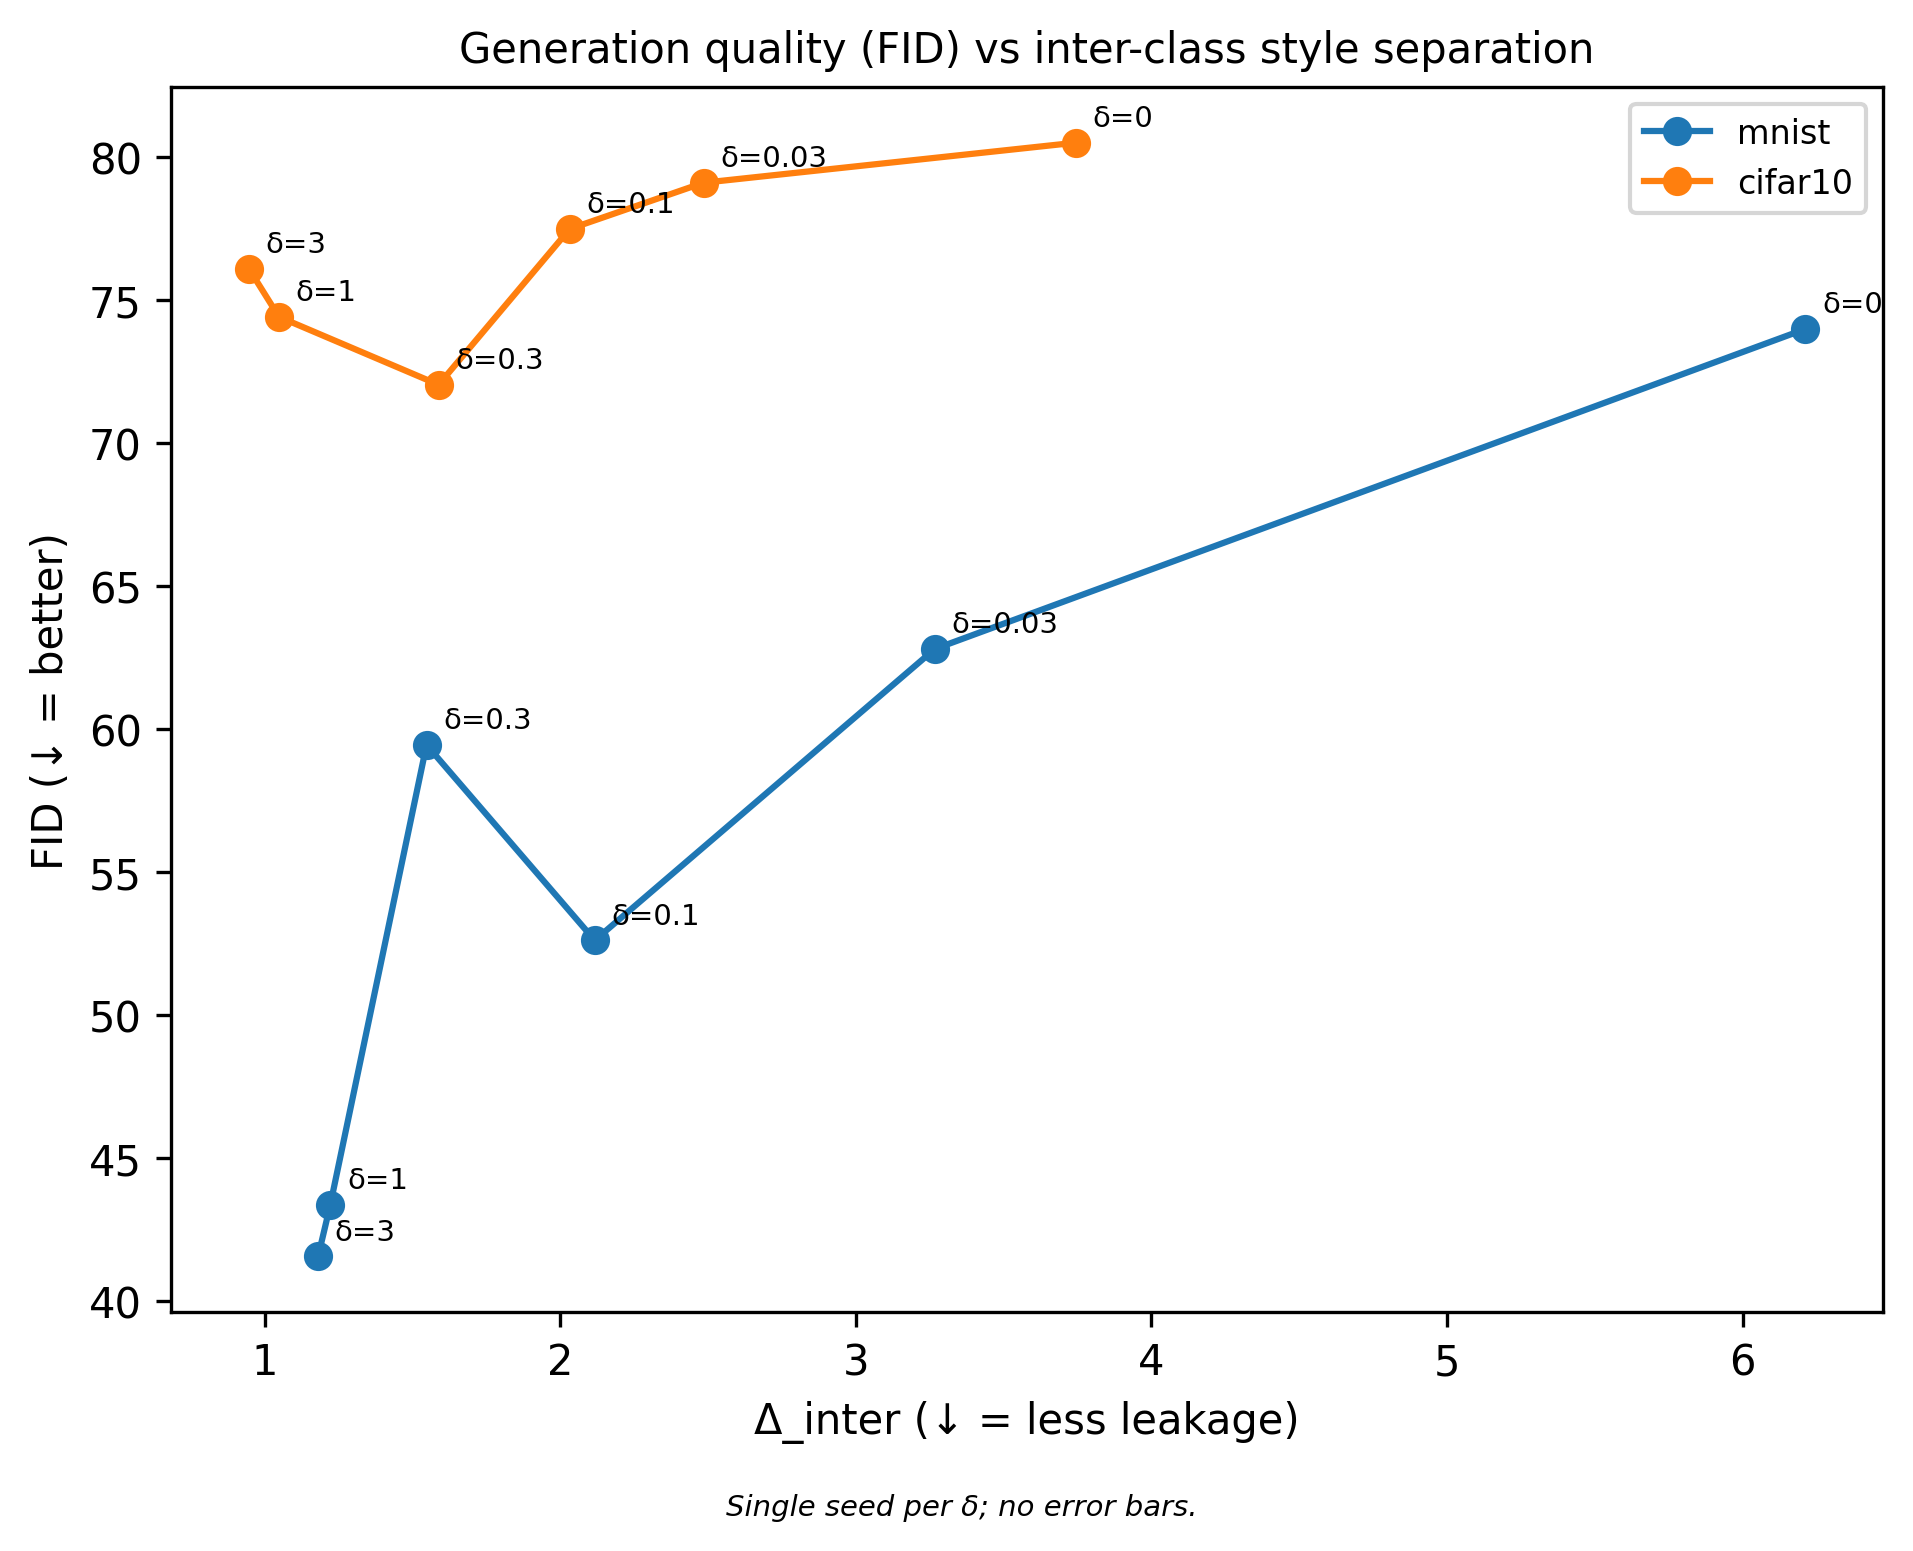
\includegraphics[width=0.55\textwidth,trim=0 0 0 65,clip]{delta_sweep_pareto_fid_deltainter.png}
\caption{Naive-prior FID against $\Dinter$ across all six single-seed
$\delta$ settings.  Connecting lines are visual aids, not claims of a smooth
response.  Conditional separation decreases steadily, whereas FID improves
overall but non-monotonically.}
\label{fig:delta-fid}
\end{figure}
\FloatBarrier

\subsection{The mismatch affects class-conditional generation}

We next test decoded samples using classifiers trained only on real pixels:
a four-layer CNN with $99.34\%$ MNIST test accuracy and a WideResNet-28-10
with $96.16\%$ CIFAR-10 test accuracy~\citep{zagoruyko2016wide}.  For a
requested class $k$, the naive sampler draws $\zc\sim p(\zc\mid k)$ and
$\zs\sim\mathcal N(0,I)$.  A post-hoc alternative fits a diagonal Gaussian
to encoded training styles from class $k$ and samples with temperature
$\tau=0.25$.  It uses labels and is a diagnostic workaround, not evidence
that the representation is disentangled.

\begin{table}[ht]
\caption{External generated-class accuracy under global and post-hoc
class-conditional style sampling.  Each checkpoint uses 50 generated images
per requested class.  CIFAR-10 is mean $\pm$ sample standard deviation over
three model seeds.}
\label{tab:generation}
\centering
\small
\begin{tabular}{lrr}
\toprule
Dataset & Global $\mathcal N(0,I)$ & Class diagonal, $\tau=0.25$ \\
\midrule
MNIST & 0.102 & 1.000 \\
CIFAR-10 & $0.132\pm0.016$ & $0.451\pm0.063$ \\
\bottomrule
\end{tabular}
\end{table}

Table~\ref{tab:generation} shows that respecting the learned
class-conditional style distribution substantially improves class identity,
especially on MNIST.  The smaller CIFAR-10 gain is consistent with a diagonal
conditional missing multimodal intra-class structure and with generally weak
sample quality; it should not be read as a complete repair.  A deterministic
mean-swap intervention also indicates that the decoder can use the style
donor's identity, but its currently archived rates use a model-internal
re-encoding evaluator.  We retain that result only as a robustness analysis
in Appendix~\ref{app:decoder}, pending the fixed external-evaluator rerun.

\begin{figure}[ht]
\centering
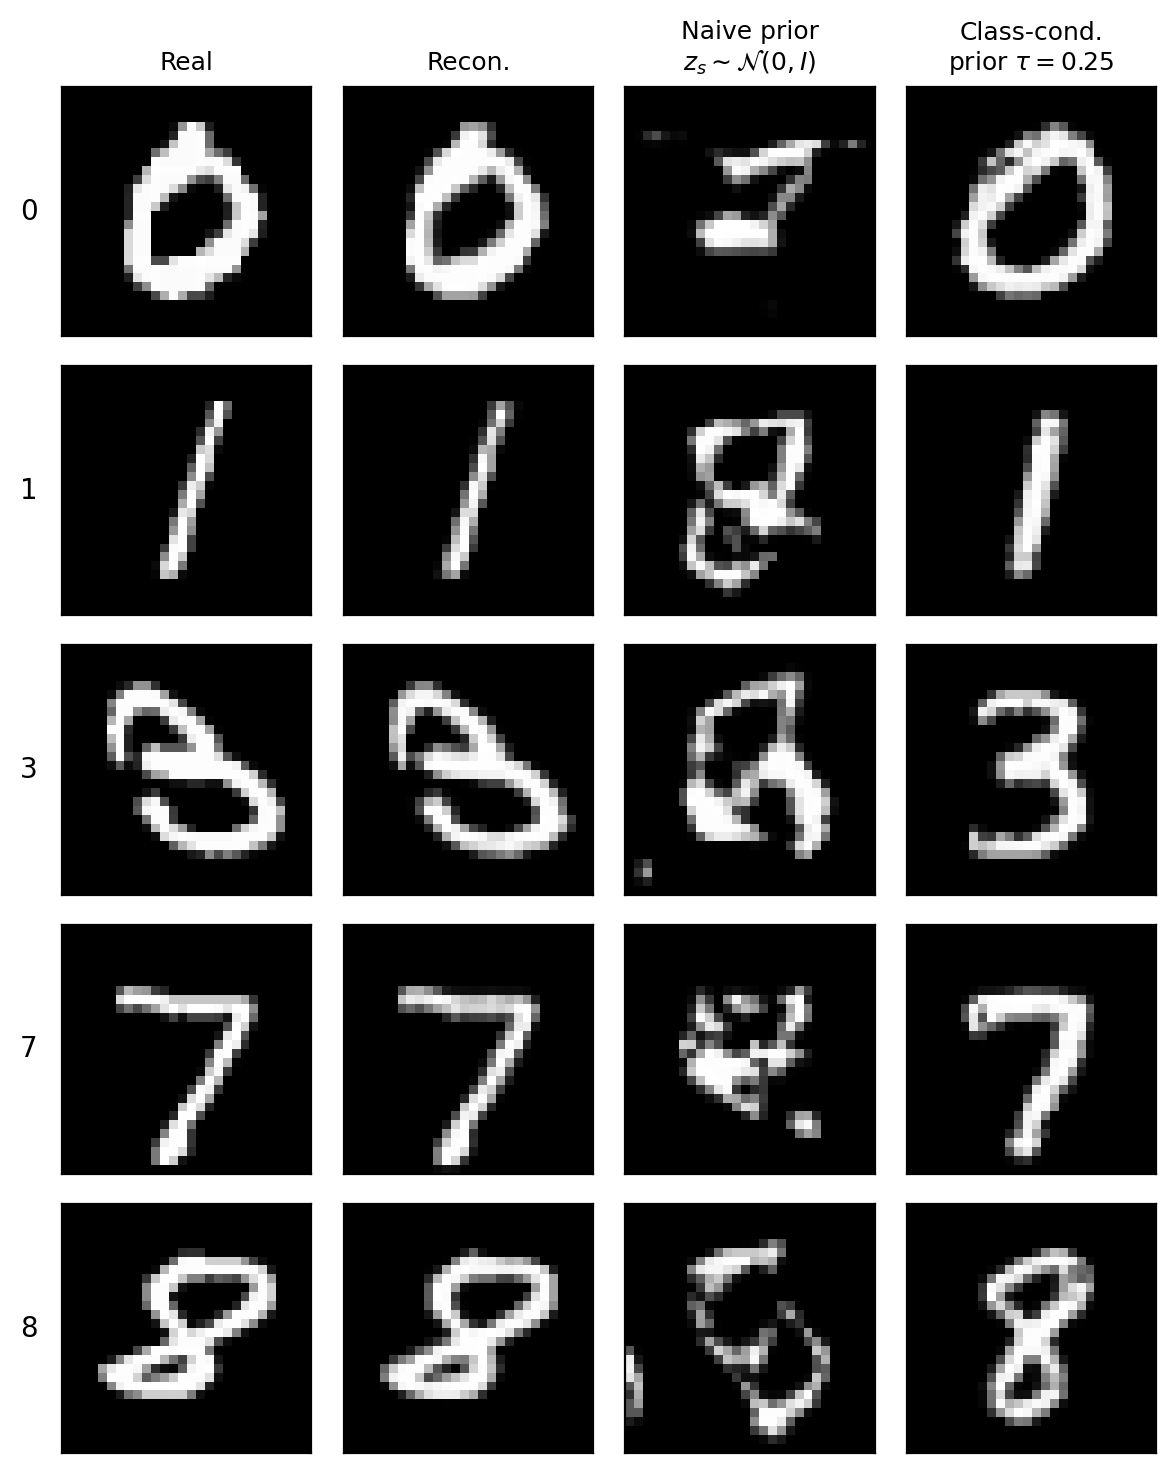
\includegraphics[width=0.43\textwidth]{mnist_recon_vs_generation_grid.png}
\caption{MNIST examples from the audited checkpoint.  Posterior
reconstructions preserve the inputs, whereas independently combining the
requested semantic prior with a global Gaussian style frequently changes
digit identity.  Fitting the style sampler conditionally restores the
requested class in these examples.  The figure is qualitative; the fixed
external evaluation is reported in Table~\ref{tab:generation}.}
\label{fig:mnist-generation}
\end{figure}

\section{Discussion and Limitations}
\label{sec:discussion}

\subsection{What the evidence chain establishes}

The decomposition separates a logically necessary condition from an
empirical failure.  Proposition~\ref{prop:nocert} shows that marginal matching
cannot certify independence in any model.  Table~\ref{tab:stage0} shows the
gap in actual stochastic posterior samples.  Table~\ref{tab:generation}
then shows that changing how style is sampled changes decoded class identity.

Each step rules out a different, weaker explanation.  The global-versus-
conditional MMD comparison rules out interpreting a small mixture-level
statistic as evidence that every class component matches the prior.  Held-out
linear and nonlinear probes, together with permutation-calibrated HSIC, show
that the discrepancy is label-structured rather than merely an arbitrary
distributional deviation.  Repeating the audit on stochastic samples rules
out a mean-only probing artifact for these checkpoints.  Finally, the
external generated-class evaluator connects the latent discrepancy to the
sampler's observable output rather than relying on re-encoded samples.  No
single diagnostic makes all four points.

The conditional-MMD intervention is supportive but deliberately secondary.
It moves conditional MMD and class-mean separation in the direction predicted
by term 2, while leaving global MMD almost unchanged.  However, its sweep is
single-seed, its quality metrics are non-monotone, and its post-hoc sampling
counterpart uses labels.  We therefore treat it as a mechanism check, not as
a new disentanglement method or a tuned remedy benchmark.

\subsection{Implications for evaluating factorized samplers}

Theorem~\ref{thm:decomp} suggests a minimal reporting standard.  First, state
the joint distribution that the decoder receives during encoding and the
distribution used at generation; otherwise the claimed factorization has no
testable contract.  Second, identify whether each diagnostic uses posterior
means, posterior samples, or prior samples.  Third, report both aggregate fit
and a conditional dependence statistic on held-out data.  Fourth, examine
within-class dependence between the proposed factors instead of stopping once
style is label-invariant.  Fifth, evaluate the final decoded samples with an
external endpoint that was not trained jointly with the generator.  The goal
is not to estimate all four KL terms, but to align each proxy with the
equality it tests.

\subsection{Limitations and threats to validity}

Several limitations bound the present evidence.  First, class labels are a
proxy for semantic content, not a complete definition of content.  Datasets
with known pose, lighting, shape, or color factors are needed to test both
directions of disentanglement.  Second, MNIST and Fashion-MNIST currently have
one model seed, while CIFAR-10 has three.  Third, the almost deterministic
style posterior may amplify leakage and motivates a controlled posterior-
entropy ablation.  Fourth, global and conditional MMD are finite-sample
kernel statistics, not KL or mutual-information estimates.  Fifth, generated
class accuracy depends on an external classifier and does not measure sample
quality or diversity.  Finally, Eq.~\ref{eq:perclass} is supervised and only
targets term 2; even perfect conditional matching would leave terms 3 and 4
unresolved.

There are also finite-sample and model-selection threats.  MMD and HSIC depend
on kernel bandwidths and have limited power in high dimension; our multiscale
kernels and permutation calibration reduce sensitivity to a single bandwidth
but do not remove it.  The probe split prevents test-set fitting, yet five
checkpoints are insufficient to characterize training variability outside
CIFAR-10.  Generated-class accuracy can be biased by the external classifier's
decision boundary, so it should be paired with precision--recall or an
equivalent diversity-sensitive measure in a definitive study.  The present
results are strongest as a falsification of the independence claim for these
checkpoints, not as an estimate of how often the failure occurs across model
families.

Our current scope is therefore an audit of a concrete factorized model, not a
claim that all architectures fail at the same magnitude.  The practical
recommendation is correspondingly narrow: when independent style sampling
requires $\zs\perp y$, report a conditional dependence test on stochastic
samples in addition to aggregate prior fit, and verify whether the decoder
uses the detected information.

\section{Conclusion}

Aggregate style matching does not license independent factorized sampling.
In \ours{}, held-out probes and permutation tests expose class information in
stochastic style samples despite small global MMD; a conditional style
sampler substantially improves generated-class accuracy.  Separating
marginal fit, conditional leakage, latent view, and decoder behavior turns
prior fit into a falsifiable sampling audit.

\clearpage
\section*{Reproducibility Statement}

Section~\ref{sec:protocol} specifies the evaluation split, latent views,
preprocessing, probe selection, and permutation calibration used for the
headline audit.  Appendix~\ref{app:proofs} contains complete proofs;
Appendix~\ref{app:model} gives the architecture, objective coefficients, and
training schedule; and Appendices~\ref{app:protocol}--\ref{app:decoder}
provide the canonical protocol, per-seed results, posterior-variance audit,
and external generation evaluation.  Appendix~\ref{app:reproducibility}
records the checkpoint and artifact boundary for every reported claim.  The
evaluation code, configurations, and result manifests will be provided as an
anonymous supplementary archive after a final identity and metadata audit.

\section*{Ethics Statement}

This work uses standard public computer-vision benchmarks and existing model
checkpoints, collects no new data, and involves no human subjects or sensitive
personal information.  Its purpose is to identify and measure a failure mode
in factorized generative models.  Generated examples are low-resolution
benchmark images; nevertheless, the broader recommendation---auditing whether
a decoder uses unintended latent information---may also help identify
representation leakage in higher-stakes applications.

\section*{AI Use Statement}

Generative AI tools were used to provide feedback on evaluation methodology
and experimental design, assist with interpretation of diagnostic results,
audit consistency between implementation artifacts and reported procedures,
and help restructure and edit the manuscript.  They were not used to generate
datasets or experimental measurements.  The authors inspected the cited
literature, verified the mathematical arguments, executed and tested the
code, checked the experimental artifacts and every reported numerical value,
and reviewed all AI-assisted text.  The authors take responsibility for the
final content of this work.

\clearpage
\IfFileExists{../iclr2027/iclr2027_conference.bst}{%
  \bibliographystyle{../iclr2027/iclr2027_conference}%
}{%
  \bibliographystyle{../iclr2026/iclr2026_conference}%
}
\bibliography{references}

\appendix
\section{Proofs}
\label{app:proofs}

\subsection{Proof of Proposition~\ref{prop:nocert}}

The label is defined after drawing $\zs$ and therefore does not alter the
marginal law of $\zs$.  Hence $q(\zs)=\mathcal N(0,I)$ and any divergence
between these two identical measures is zero.  Because $y$ is a deterministic
function of $\zs$, $H(y\mid\zs)=0$.  The equal-probability partition gives
$H(y)=\log K$, and consequently
$I(\zs;y)=H(y)-H(y\mid\zs)=\log K$.

\subsection{A smooth, full-support construction}

Let $z\sim\mathcal N(0,1)$ and, conditional on $z$, draw a binary label with
\begin{equation}
P(y=1\mid z)=\sigma(az),\qquad P(y=0\mid z)=\sigma(-az),
\end{equation}
where $a>0$ and $\sigma(t)=(1+e^{-t})^{-1}$.  Since the standard normal
density $\phi$ is symmetric and $\sigma(t)+\sigma(-t)=1$,
\begin{align}
P(y=1)
&=\int_{\mathbb R}\phi(z)\sigma(az)\,dz\\
&=\frac12\int_{\mathbb R}\phi(z)
\bigl[\sigma(az)+\sigma(-az)\bigr]\,dz=\frac12.
\end{align}
The generative construction starts with the standard normal and changes only
the conditional label law, so the marginal of $z$ remains exactly standard
normal.  Bayes' rule gives
\begin{equation}
q(z\mid y=1)=2\phi(z)\sigma(az),\qquad
q(z\mid y=0)=2\phi(z)\sigma(-az).
\end{equation}
Both densities are smooth and strictly positive on $\mathbb R$.  When
$a\rightarrow\infty$, the conditional label approaches the indicator of the
sign of $z$ outside a set of Gaussian measure zero.  Thus
$H(y\mid z)\rightarrow0$ and $I(z;y)\rightarrow\log2$ while the marginal
remains unchanged.

\subsection{Proof of Theorem~\ref{thm:decomp}}

For a fixed $y$, insert the product of the encoder conditionals and apply the
KL chain rule:
\begin{align}
&\KL\!\left(q(\zc,\zs\mid y)\|p(\zc\mid y)p(\zs)\right)\\
={}&\KL\!\left(q(\zc,\zs\mid y)\|q(\zc\mid y)q(\zs\mid y)\right)\nonumber\\
&+\KL(q(\zc\mid y)\|p(\zc\mid y))
+\KL(q(\zs\mid y)\|p(\zs)).
\end{align}
The first term is $I_q(\zc;\zs\mid y)$ at that label.  Averaging over
$q(y)$ gives term 4 and term 3 of Eq.~\ref{eq:decomp}.  For the last term,
insert the aggregate posterior $q(\zs)$:
\begin{align}
\mathbb E_{q(y)}\KL(q(\zs\mid y)\|p(\zs))
={}&\mathbb E_{q(y)}\KL(q(\zs\mid y)\|q(\zs))\nonumber\\
&+\KL(q(\zs)\|p(\zs))\\
={}&I_q(\zs;y)+\KL(q(\zs)\|p(\zs)).
\end{align}
This establishes the equality for arbitrary $q(y)$.  Non-negativity follows
from non-negativity of KL divergence and mutual information.

\subsection{Proof of Corollary~\ref{cor:valid}}

An expectation of a non-negative KL is zero iff its integrand is zero for
$q(y)$-almost every $y$, which holds iff the two latent conditional measures
are equal.  The pushforward inequality follows by applying the data-processing
inequality to the deterministic Markov kernel induced by the decoder for each
$y$, then averaging over $q(y)$.

\section{Architecture and Training}
\label{app:model}

\subsection{Architecture}

The shared encoder is a ResNet-18 adapted to small images: its first
$7\times7$, stride-2 convolution is replaced by a $3\times3$, stride-1
convolution and max pooling is removed.  The trunk output is flattened and
mapped to 256 dimensions with SiLU.  Separate heads produce an unnormalized
semantic direction, a scalar semantic concentration, a style mean, and a
style log variance.  We use
\begin{align}
\muc&=\widetilde\muc/\|\widetilde\muc\|_2, &
\rho_c&=\sigma(r_c)(1-\varepsilon),\\
\zs&=\mus+\exp(\tfrac12\log\sigma_s^2)\odot\epsilon,
&\epsilon&\sim\mathcal N(0,I).
\end{align}
The semantic code is sampled by a Spherical Cauchy M\"obius
reparameterization.  The decoder concatenates $[\zc;\zs]$, projects it to a
$512\times4\times4$ tensor, and applies three residual bilinear-upsample
blocks with channel widths $256,128,64$.  Its sigmoid output is interpolated
to the native dataset resolution when necessary.  MNIST and Fashion-MNIST
therefore remain $28\times28$ and single-channel; CIFAR-10 remains
$32\times32\times3$.

For class $k$, the semantic prior is a Spherical Cauchy distribution centered
at an EMA direction $m_k$, with concentration $\rho_p=0.7$.  The center is
updated once per epoch from encoded class-mean directions with momentum
$0.95$.  The style prior is $\mathcal N(0,I)$.

\subsection{Objective}

The training objective is
\begin{align}
\mathcal L={}&\mathcal L_{\mathrm{rec}}
+\alpha(t)\mathcal L_{\mathrm{class}}
+\beta(t)\mathcal L_{\mathrm{agg}}
+\gamma(t)\mathcal L_{\mathrm{style}}\nonumber\\
&+\delta(t)\mathcal L_{\mathrm{style-cls}}
+\eta(t)\mathcal L_{\mathrm{cls}}.
\end{align}
$\mathcal L_{\mathrm{rec}}$ is L1 plus $0.1$ LPIPS
\citep{zhang2018unreasonable}.  $\mathcal L_{\mathrm{class}}$ matches each
semantic class conditional to its spherical prior, $\mathcal L_{\mathrm{agg}}$
matches aggregate semantic codes to the class-prior mixture,
$\mathcal L_{\mathrm{style}}$ matches sampled style codes to a standard
Gaussian, and $\mathcal L_{\mathrm{cls}}$ is cross entropy from $\muc$.
The baseline checkpoints audited in the main paper explicitly set
$\delta=0$; the repository default for new remedied runs is $\delta=1$, so
the run manifest or command-line override is required to distinguish them.

\begin{table}[ht]
\caption{Case-study training hyperparameters.}
\label{tab:hyperparameters}
\centering
\small
\begin{tabular}{ll}
\toprule
Parameter & Value \\
\midrule
Optimizer & Adam, learning rate $10^{-3}$ \\
Schedule & StepLR, step 100, factor $0.5$ \\
Batch size / epochs & 128 / 300 \\
Gradient clipping & global norm 1.0 \\
Semantic / style dimension & 64 / 128 \\
Semantic-prior concentration & 0.7 \\
EMA momentum & 0.95 \\
Final class / aggregate MMD weights & 2.0 / 5.0 \\
Final global style MMD weight & 1.0 \\
Final auxiliary-classifier weight & 0.3 \\
\bottomrule
\end{tabular}
\end{table}

Training has four phases: reconstruction only for epochs 0--49; global style
MMD and the auxiliary classifier ramp during epochs 50--99; semantic class
and aggregate MMD ramp to half strength during epochs 100--199; all terms
reach full strength during epochs 200--299.  For remedied runs, per-class
style MMD follows the global-style ramp.  No image augmentation is used.

\section{Canonical Audit Protocol}
\label{app:protocol}

\subsection{Data split and latent views}

For each checkpoint we select 2,048 examples from the standard test split
with evaluation seed 0.  Probe indices are generated by a deterministic
stratified 60/20/20 split, yielding 1,228 training, 410 validation, and 410
test examples.  Standardization parameters are estimated only on the 1,228
probe-training examples.  The split indices are stored by SHA-256 hash in
each result manifest.

The encoder is evaluated once to obtain $(\muc,\mus,\log\sigma_s^2)$ and a
seeded stochastic draw $\zs$.  We use:
\begin{itemize}
    \item $\mus$ for representation probes and deterministic mean swaps;
    \item $\zs$ for global MMD, conditional style statistics, and the
    sampling-contract probe; and
    \item $(\muc,\mus)$ for the currently available mean-view conditional
    dependence diagnostic.
\end{itemize}
Agreement between these views is reported as an empirical result rather than
assumed.

\subsection{Probe suite}

The suite contains multinomial logistic regression, a fixed two-layer MLP,
RBF-SVM, and $k$-NN.  Validation data are used for fixed early-stopping or
model-selection rules; every headline accuracy is evaluated once on the
untouched test partition.  We report accuracy and macro-F1.  The main paper
uses logistic regression as the simplest standardized headline and includes
RBF-SVM to detect nonlinear separation.

\subsection{MMD and HSIC}

Global MMD is the unbiased U-statistic with the averaged Euclidean RBF kernel
\begin{equation}
k(u,v)=\frac17\sum_{\sigma\in\{0.5,1,2,5,10,20,50\}}
\exp\!\left(-\frac{\|u-v\|_2^2}{2\sigma^2}\right).
\end{equation}
The Gaussian reference has the same sample count as the encoded set.
$\Dinter$ is not an MMD; it is the average Euclidean distance between all
pairs of class-conditional style means.

HSIC centers a multiscale style Gram matrix and a label Gram matrix and uses
1,024 examples for bounded memory.  We calibrate it by 200 label
permutations.  With the plus-one correction,
\begin{equation}
p=\frac{1+\#\{T_b\ge T_{\mathrm{obs}}\}}{201},
\end{equation}
so $p=0.004975$ is reported rather than $p=0$.  Conditional HSIC for term 4
permutes styles independently inside every represented class.

We do not report the current JointMMD U-statistic as a headline result.  Its
joint and recombined samples share observations, so the nominal independent
two-sample U-statistic assumptions require a sample-splitting calibration
that is not yet part of the canonical protocol.

\section{Full Stage-0 Results}
\label{app:full-results}

\begin{table}[ht]
\caption{Full held-out probe suite.  Values are test accuracy in percent.
CIFAR-10 is mean $\pm$ sample standard deviation over model seeds 0, 1, 2.}
\label{tab:full-probes}
\centering
\small
\begin{tabular}{llrrrr}
\toprule
Dataset & View & Logistic & MLP & RBF-SVM & $k$-NN \\
\midrule
MNIST & $\mus$ & 99.76 & 99.51 & 99.76 & 97.80 \\
      & $\zs$  & 99.76 & 99.51 & 99.76 & 97.80 \\
Fashion & $\mus$ & 88.29 & 90.73 & 93.17 & 85.12 \\
        & $\zs$  & 88.29 & 90.73 & 93.17 & 85.61 \\
CIFAR-10 & $\mus$ & $68.46\pm6.29$ & $70.49\pm3.83$ &
$70.24\pm3.23$ & $42.52\pm6.93$ \\
         & $\zs$ & $68.62\pm6.19$ & $70.57\pm3.50$ &
$70.16\pm3.36$ & $42.20\pm7.11$ \\
\bottomrule
\end{tabular}
\end{table}

\begin{table}[ht]
\caption{Per-seed CIFAR-10 results for the two principal probes.}
\label{tab:cifar-seeds}
\centering
\small
\begin{tabular}{lrrrrr}
\toprule
Seed & $\Dinter(\zs)$ & Logit $\mus$ & Logit $\zs$ & RBF $\mus$ & RBF $\zs$ \\
\midrule
0 & 3.801 & 61.46 & 61.71 & 66.59 & 66.34 \\
1 & 4.264 & 73.66 & 73.66 & 72.68 & 72.68 \\
2 & 3.797 & 70.24 & 70.49 & 71.46 & 71.46 \\
\bottomrule
\end{tabular}
\end{table}

The classwise conditional-HSIC mean-view statistic is 0.002440 on MNIST,
0.002459 on Fashion-MNIST, and $0.002086\pm0.000222$ on CIFAR-10.  Every
checkpoint attains the minimum calibrated $p=1/201$.  We interpret this as
evidence of within-class dependence in the deterministic representation,
not as a numerical estimate of $I(\zc;\zs\mid y)$.

\subsection{Structure of the conditional mismatch}

The class average in Table~\ref{tab:conditional-mmd} compresses a structured
ten-class discrepancy.  Figure~\ref{fig:pairwise-mmd-app} compares every
pair of class-conditional style distributions.  Broad off-diagonal mass is
visible on both datasets, rather than separation being confined to a few
class pairs.  These matrices use the same stochastic-view diagnostic as the
per-class prior comparison; their scale should not be compared across
datasets as if it were a normalized dependence measure.

\begin{figure}[t]
\centering
\begin{minipage}{0.47\textwidth}
\centering
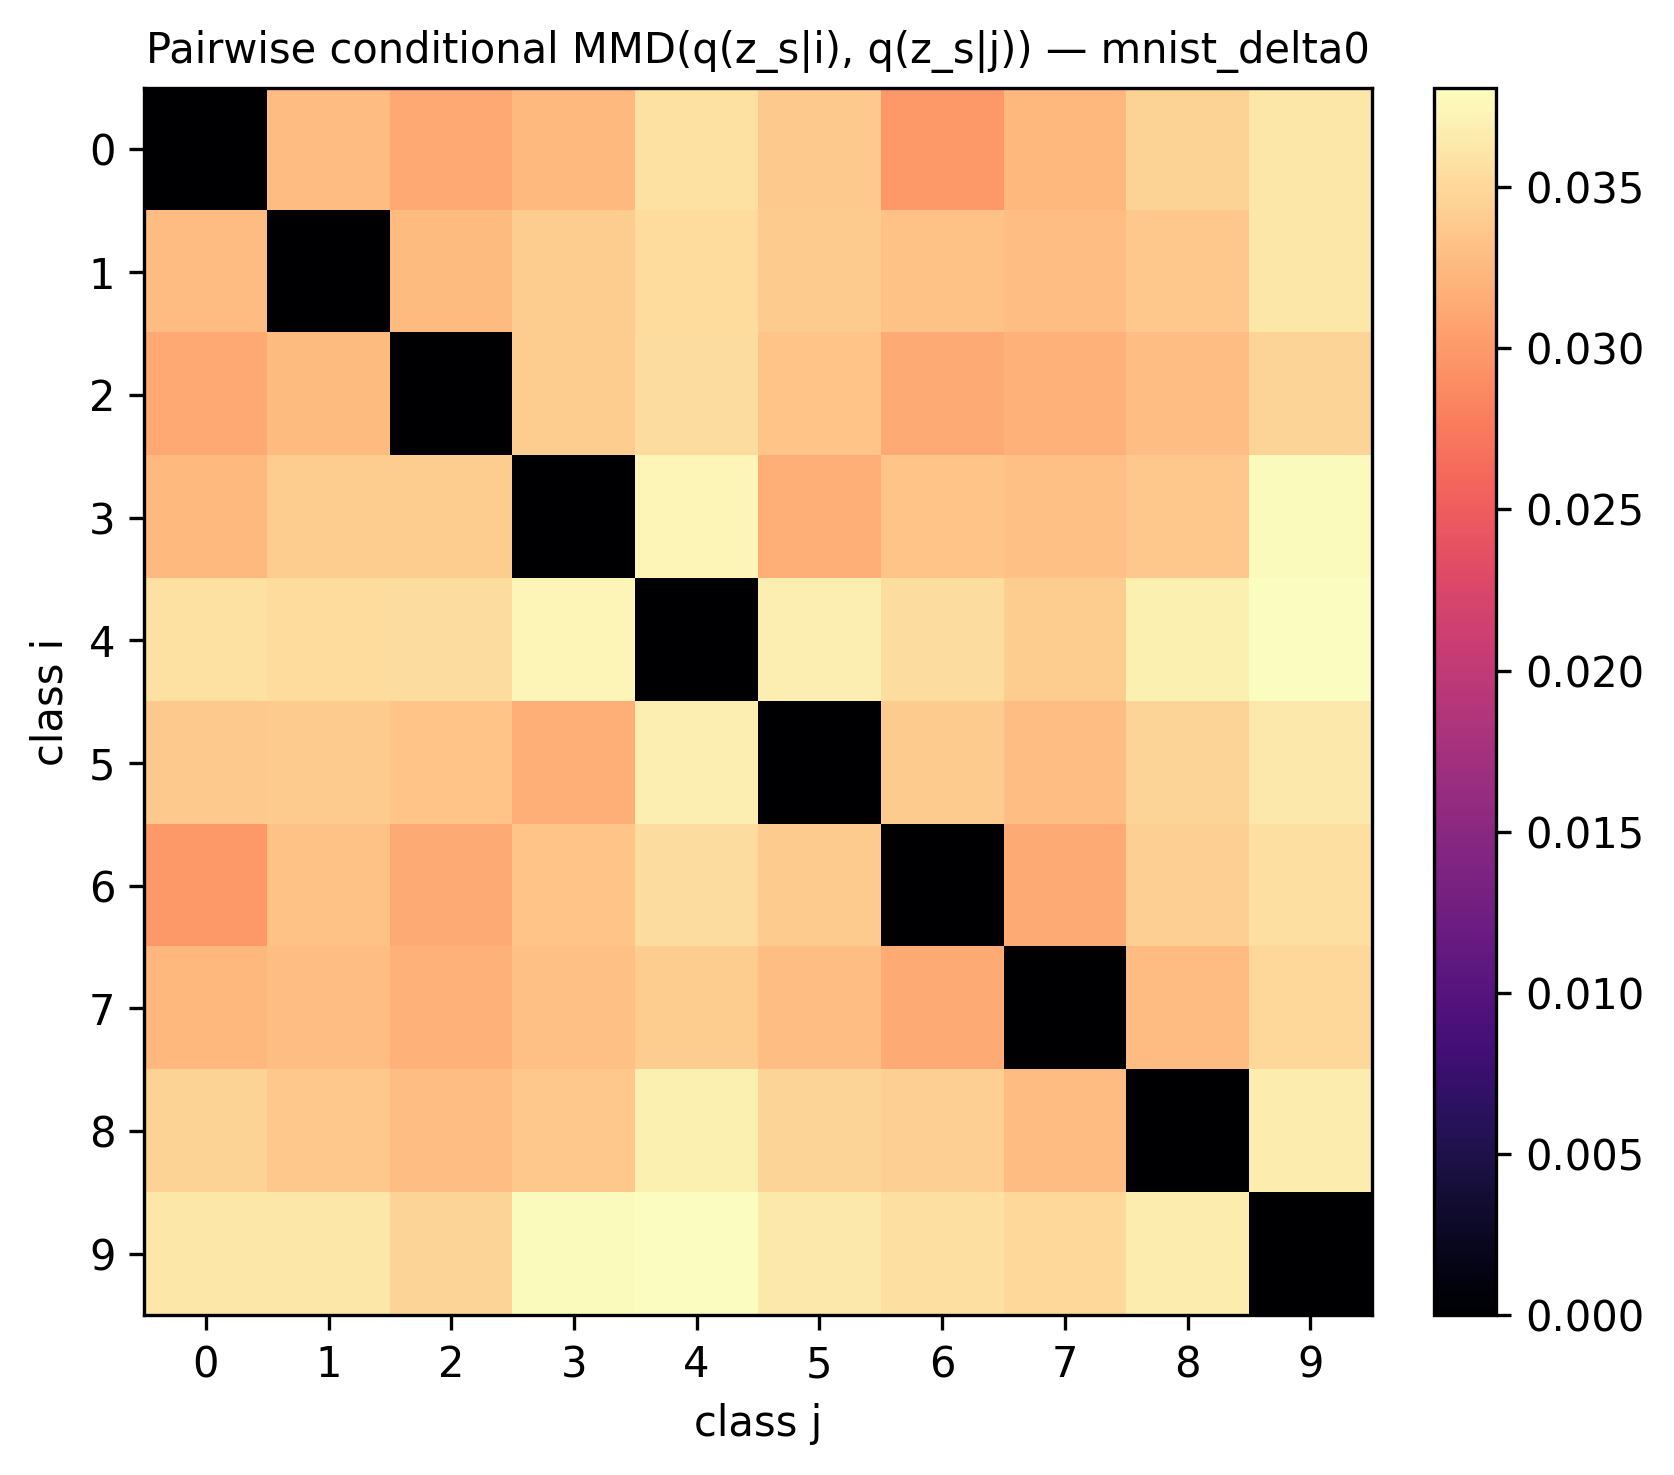
\includegraphics[width=\linewidth,trim=0 0 0 70,clip]{conditional_mmd_pairwise_heatmap_mnist.png}\\[-0.4em]
\small (a) MNIST
\end{minipage}\hfill
\begin{minipage}{0.47\textwidth}
\centering
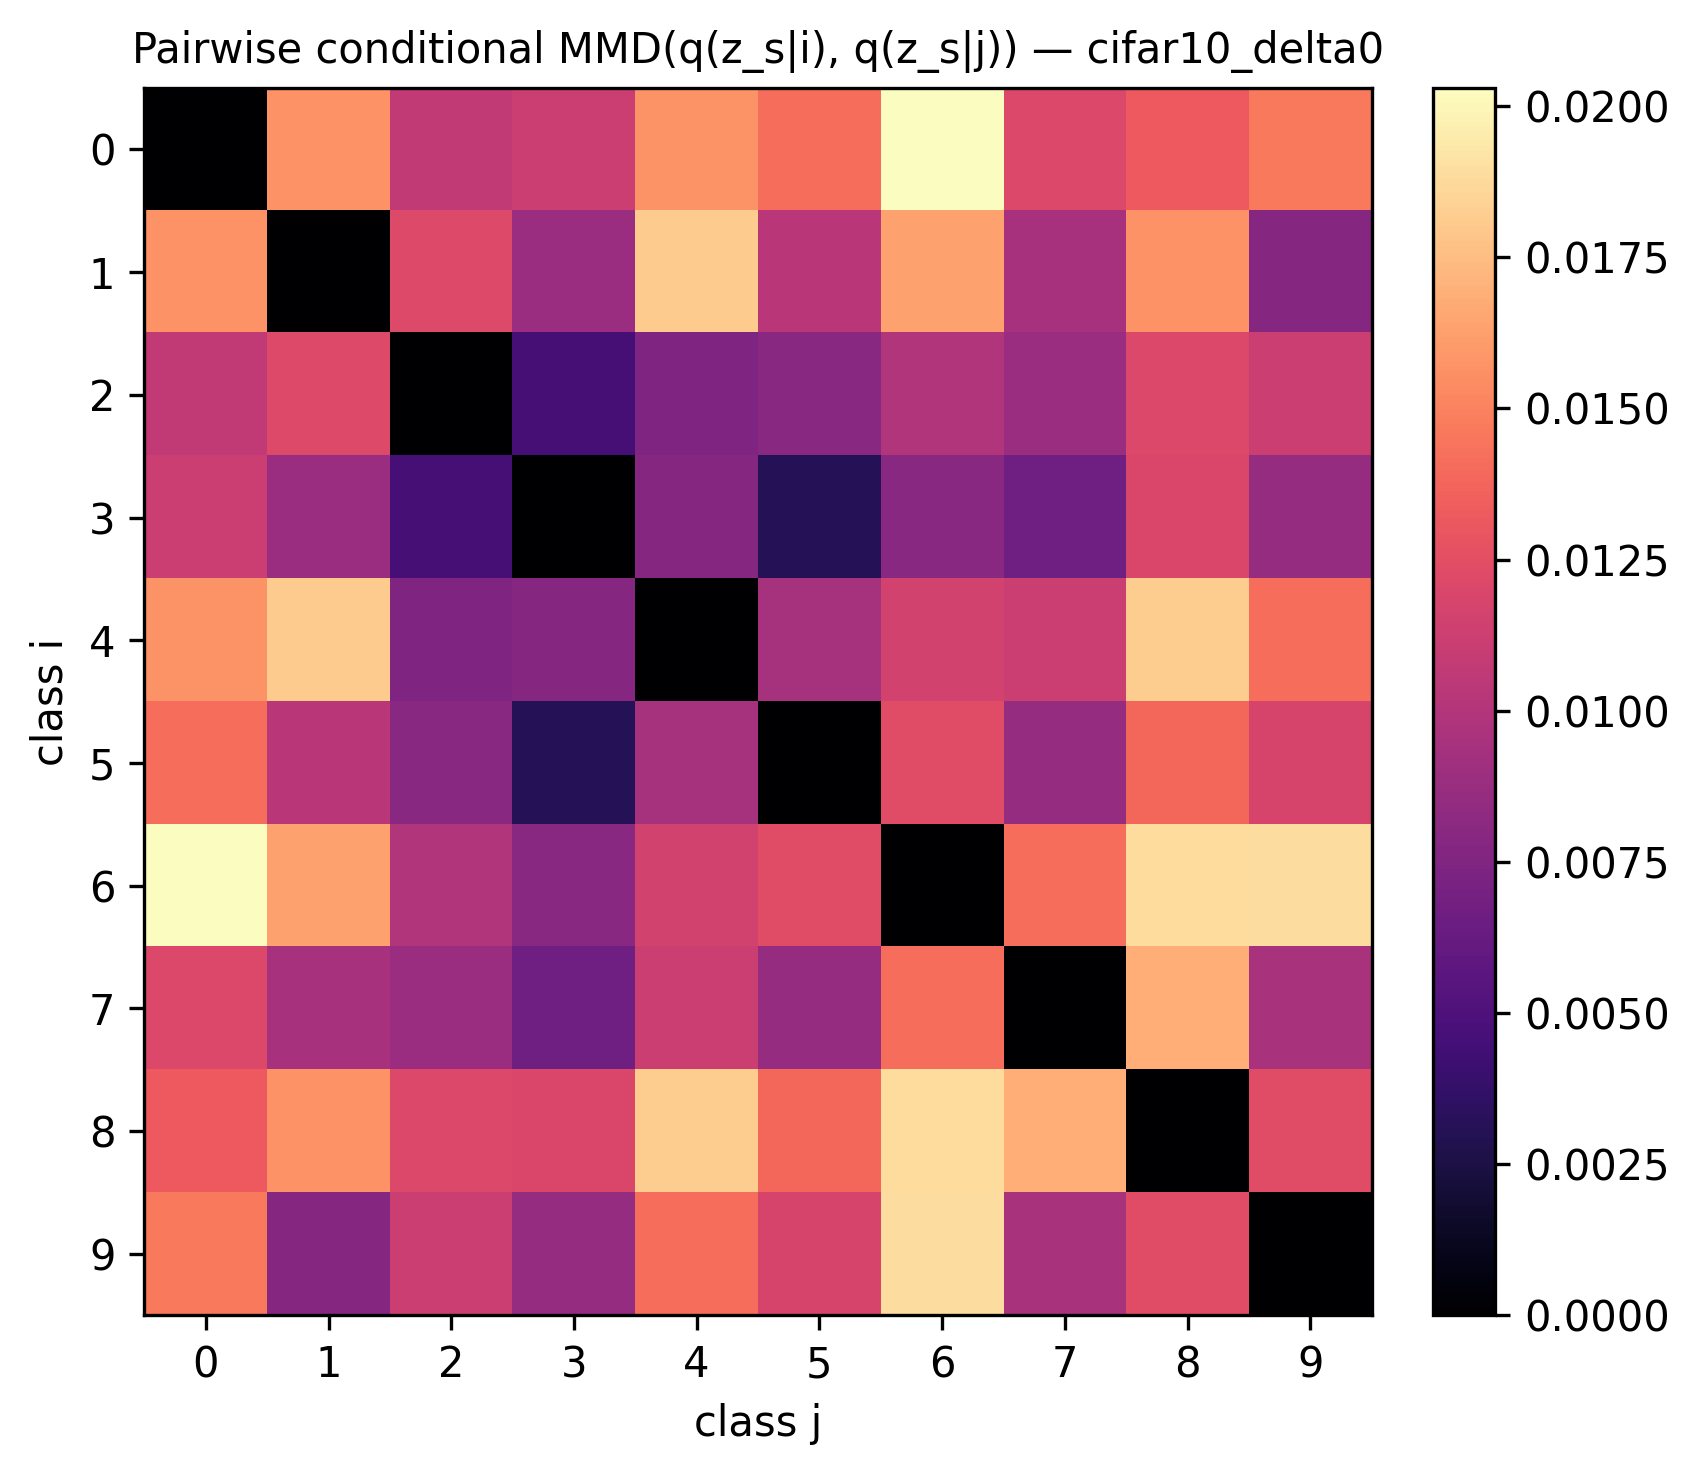
\includegraphics[width=\linewidth,trim=0 0 0 70,clip]{conditional_mmd_pairwise_heatmap_cifar10.png}\\[-0.4em]
\small (b) CIFAR-10
\end{minipage}
\caption{Pairwise $\MMD^2(q(\zs\mid y=i),q(\zs\mid y=j))$ for the
unrepaired seed-0 checkpoints.  The diagonal is zero by construction;
off-diagonal structure shows that conditional style distributions differ
throughout the label set.}
\label{fig:pairwise-mmd-app}
\end{figure}

Figure~\ref{fig:projection-app} gives a complementary one-dimensional view.
The projection direction is computed from the class means rather than chosen
after inspecting individual examples.  Several MNIST classes separate along
this direction, but the overlap also illustrates why a single projection is
not a substitute for the held-out multivariate probes.

\begin{figure}[t]
\centering
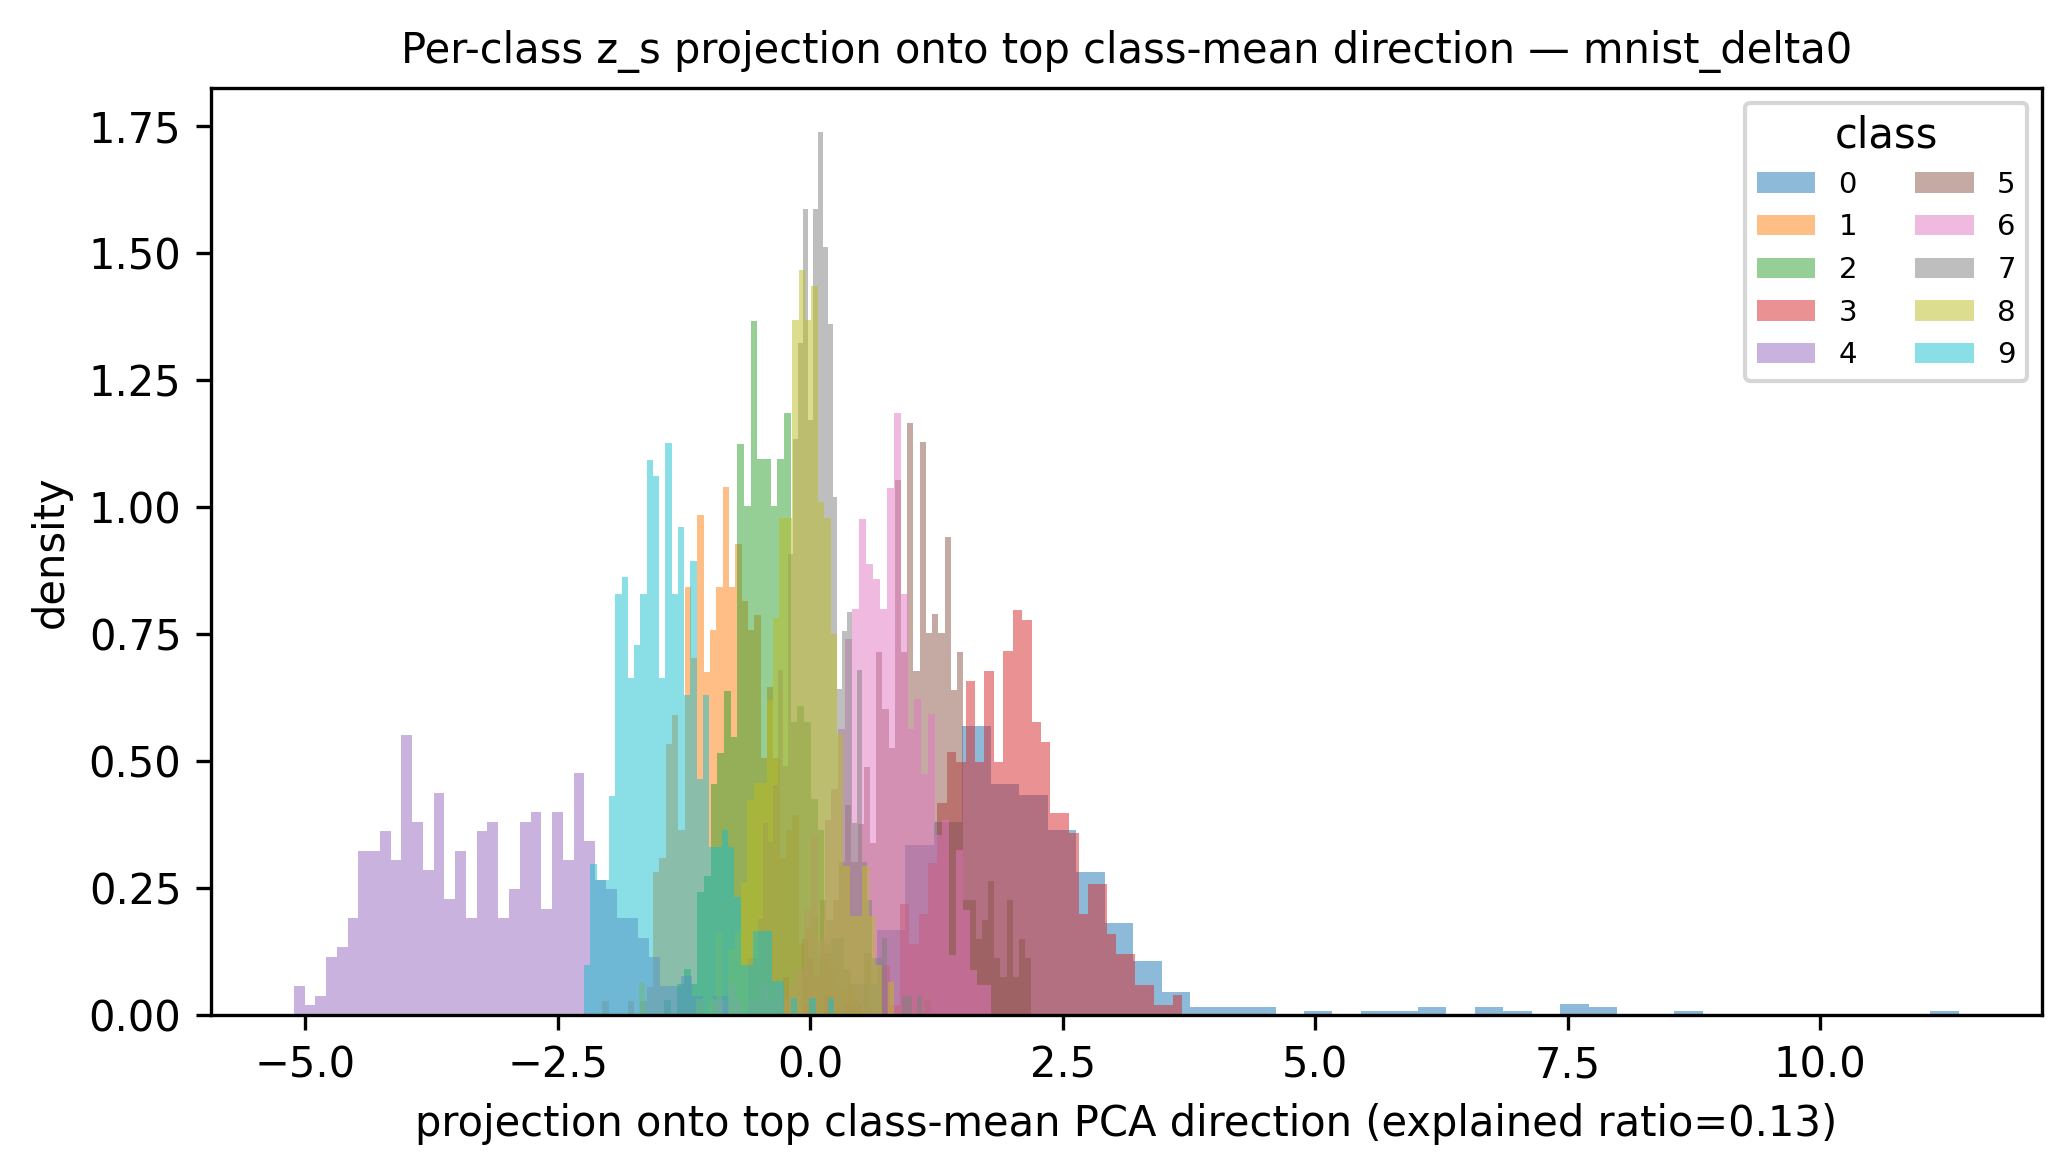
\includegraphics[width=0.78\textwidth,trim=0 0 0 80,clip]{conditional_mmd_projection_histogram_mnist.png}
\caption{MNIST stochastic styles projected onto the leading direction of
the class-mean matrix at $\delta=0$.  The direction explains 13.1\% of the
class-mean variance.  The plot is descriptive; the held-out probes and HSIC
tests provide the quantitative evidence.}
\label{fig:projection-app}
\end{figure}
\FloatBarrier

\subsection{Posterior-variance inspection}

The fractions of raw style log-variance coordinates at or below the clamp
floor are 99.9966\% (MNIST), 99.9989\% (Fashion-MNIST), and 100\% for all
three CIFAR-10 checkpoints.  Because this statistic was added during the
post-hoc checkpoint audit, it is reported in the human-readable audit report;
future manifests should also store it as a first-class numeric field.

\subsection{Complete conditional-regularization sweep}

Table~\ref{tab:full-delta-sweep} expands the four points shown in the main
paper to all six archived $\delta$ settings.  We retain ACC, $\Dinter$, and
FID because they are directly tied to the sweep artifacts, but omit the
historical probe column until it is regenerated with the canonical held-out
split.  Each point is a separate single-seed training run.

\begin{table}[ht]
\caption{Complete single-seed per-class-style-MMD sweep.  Lower FID and
$\Dinter$ are better; no uncertainty or significance claim is made.}
\label{tab:full-delta-sweep}
\centering
\small
\setlength{\tabcolsep}{4pt}
\begin{tabular}{lrrrrrr}
\toprule
& \multicolumn{3}{c}{MNIST} & \multicolumn{3}{c}{CIFAR-10} \\
$\delta$ & ACC & $\Dinter$ & FID & ACC & $\Dinter$ & FID \\
\midrule
0    & .9915 & 6.21 & 74.0 & .8129 & 3.74 & 80.5 \\
.03  & .9944 & 3.27 & 62.8 & .8111 & 2.48 & 79.1 \\
.1   & .9898 & 2.12 & 52.6 & .8100 & 2.03 & 77.5 \\
.3   & .9936 & 1.55 & 59.4 & .7148 & 1.59 & 72.0 \\
1    & .8592 & 1.22 & 43.4 & .8000 & 1.05 & 74.4 \\
3    & .9929 & 1.18 & 41.5 & .7994 & .95  & 76.1 \\
\bottomrule
\end{tabular}
\end{table}

\FloatBarrier

\section{Generation and Decoder Diagnostics}
\label{app:decoder}

\subsection{External generation evaluation}

The independent MNIST evaluator is a four-convolution CNN trained for 20
epochs on real images only.  Its standard test accuracy is 99.34\%.  The
CIFAR-10 evaluator is a WideResNet-28-10 trained for 200 epochs with standard
random-crop and horizontal-flip augmentation on real training images only;
its test accuracy is 96.16\%.  Neither evaluator contributes to the
generative model's loss.

\begin{table}[ht]
\caption{Per-checkpoint external Gen-ACC.  Each entry uses 50 images per
requested class.}
\label{tab:generation-seeds}
\centering
\small
\begin{tabular}{llrr}
\toprule
Dataset & Model seed & Global Gaussian & Class diagonal $\tau=.25$ \\
\midrule
MNIST & 0 & 0.102 & 1.000 \\
CIFAR-10 & 0 & 0.138 & 0.390 \\
CIFAR-10 & 1 & 0.144 & 0.516 \\
CIFAR-10 & 2 & 0.114 & 0.448 \\
\bottomrule
\end{tabular}
\end{table}

The class-diagonal distribution is fit from encoded training styles and
therefore deliberately conditions style on the requested label.  Its gain
tests whether the decoder is sensitive to the conditional mismatch.  It is
not an unconditional generative model and does not repair the encoder.

Figure~\ref{fig:cifar-sampling-app} displays the qualitative counterpart of
Table~\ref{tab:generation-seeds}.  Conditioning style makes the requested
category more visually consistent in some rows, but shrinking the diagonal
Gaussian to $\tau=.25$ also reduces variation and can produce blurry or
prototype-like outputs.  This is why Gen-ACC is interpreted jointly with FID
and not as a stand-alone measure of generative quality.

\begin{figure}[t]
\centering
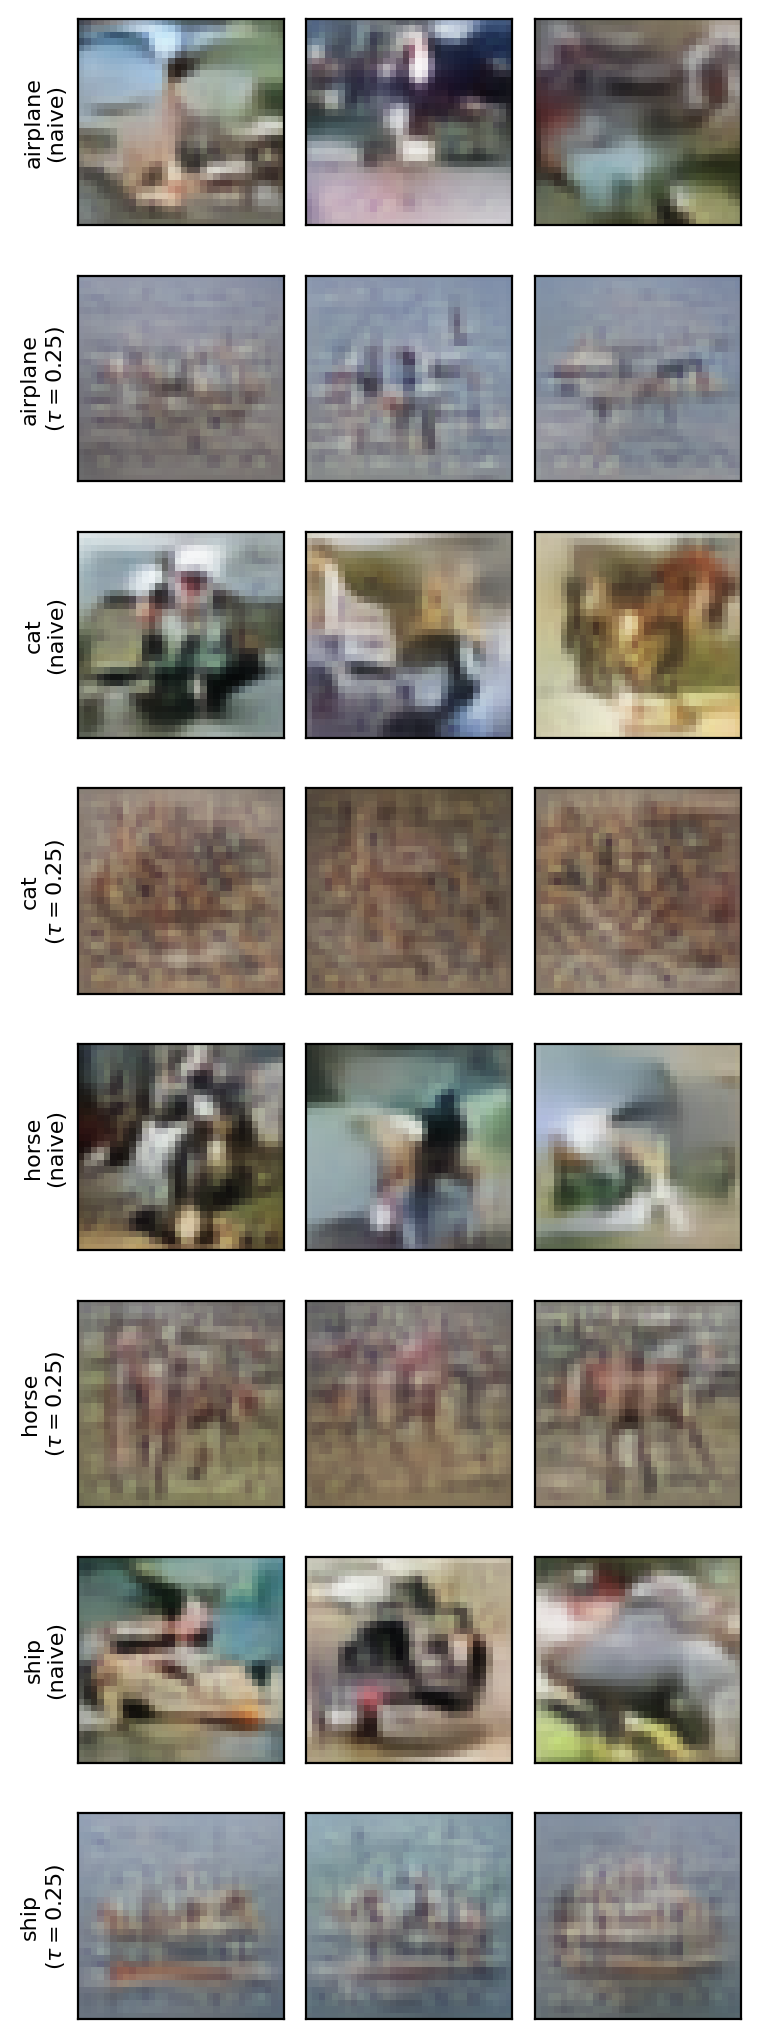
\includegraphics[width=0.43\textwidth]{cifar10_sampling_grid_trimmed.png}
\caption{Archived CIFAR-10 samples from the seed-0 checkpoint.  For four
requested classes, odd rows use the global Gaussian style prior and even rows
use the post-hoc class-diagonal prior at $\tau=.25$.  The grid is qualitative;
external Gen-ACC is reported in Table~\ref{tab:generation-seeds}.}
\label{fig:cifar-sampling-app}
\end{figure}
\FloatBarrier

\subsection{Archived deterministic mean-swap analysis}

For each ordered pair of distinct classes $(a,b)$, the archived diagnostic
decodes $\mathrm{Dec}(\muc^{(a)},\mus^{(b)})$ for 100 independent donor pairs.
On the unrepaired checkpoint, the model-internal re-encoding classifier
follows the style donor on 99.22\% of MNIST and 68.82\% of CIFAR-10
off-diagonal swaps, while following the semantic donor on 0.11\% and 4.22\%.
These values support the same qualitative mechanism but are not primary
evidence because the evaluator shares the model's semantic representation.
They will be replaced by the independent pixel-classifier rerun before being
promoted to the main paper.

\begin{figure}[t]
\centering
\begin{minipage}{0.48\textwidth}
\centering
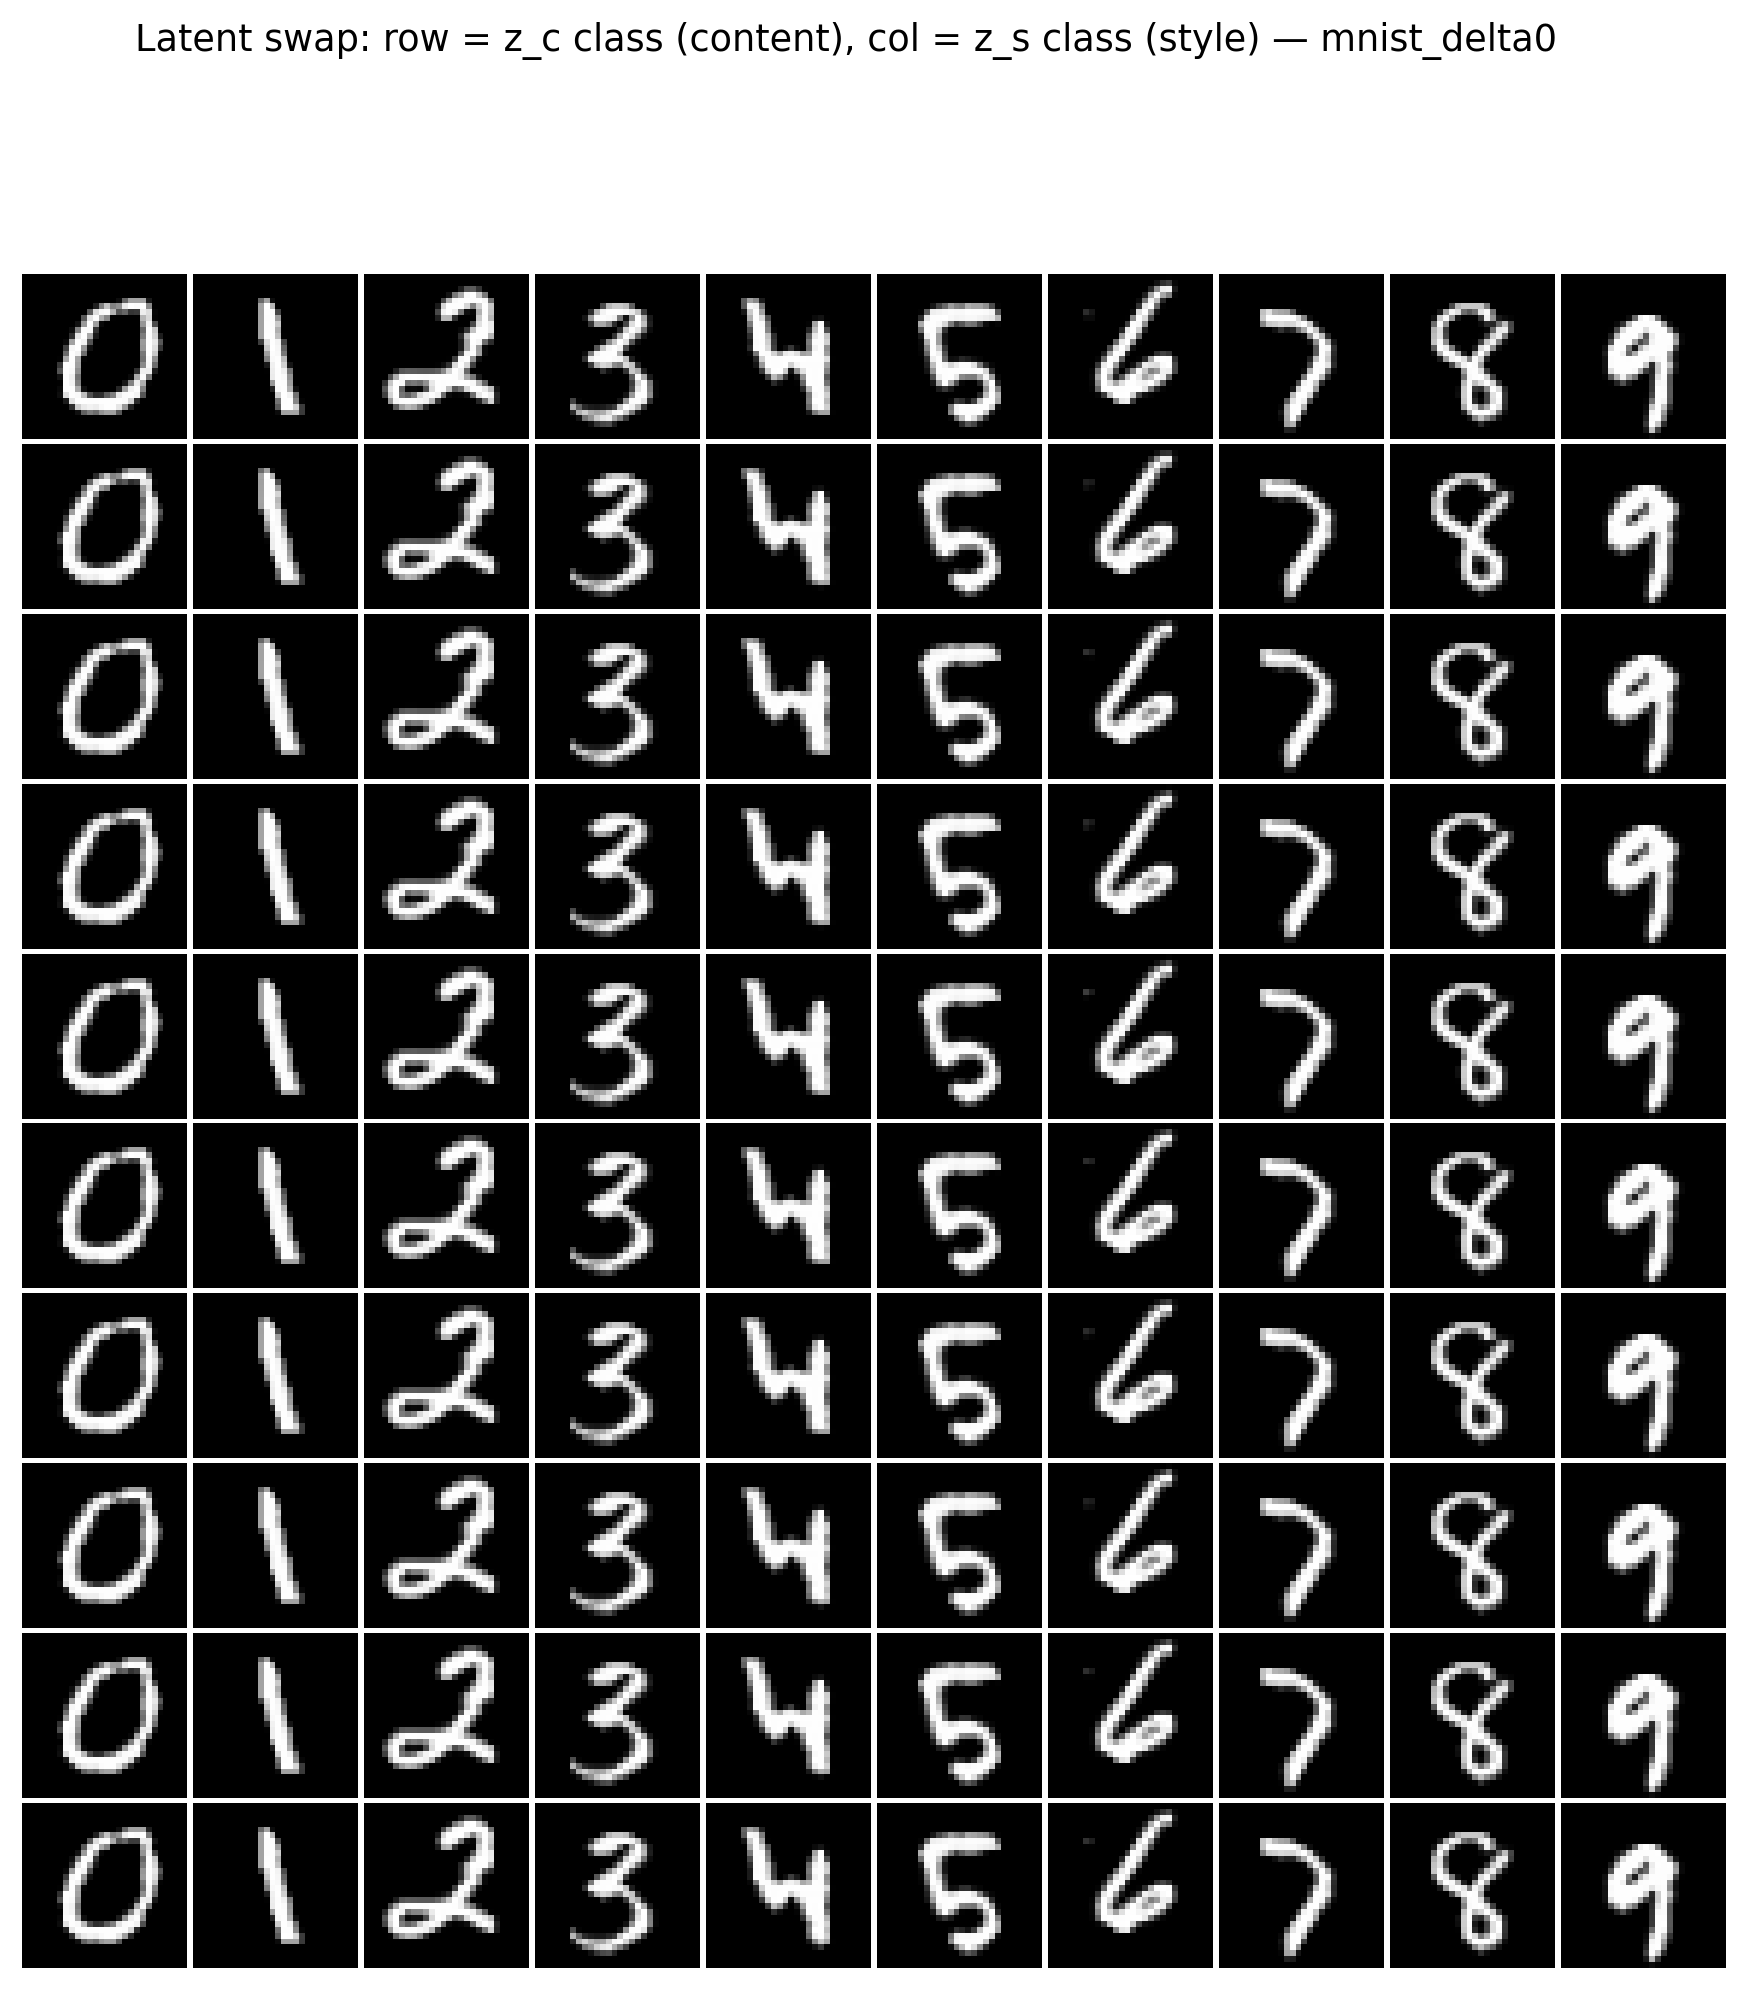
\includegraphics[width=0.86\linewidth]{mnist_swap_grid_delta0.png}\\[-0.4em]
\small (a) MNIST
\end{minipage}\hfill
\begin{minipage}{0.48\textwidth}
\centering
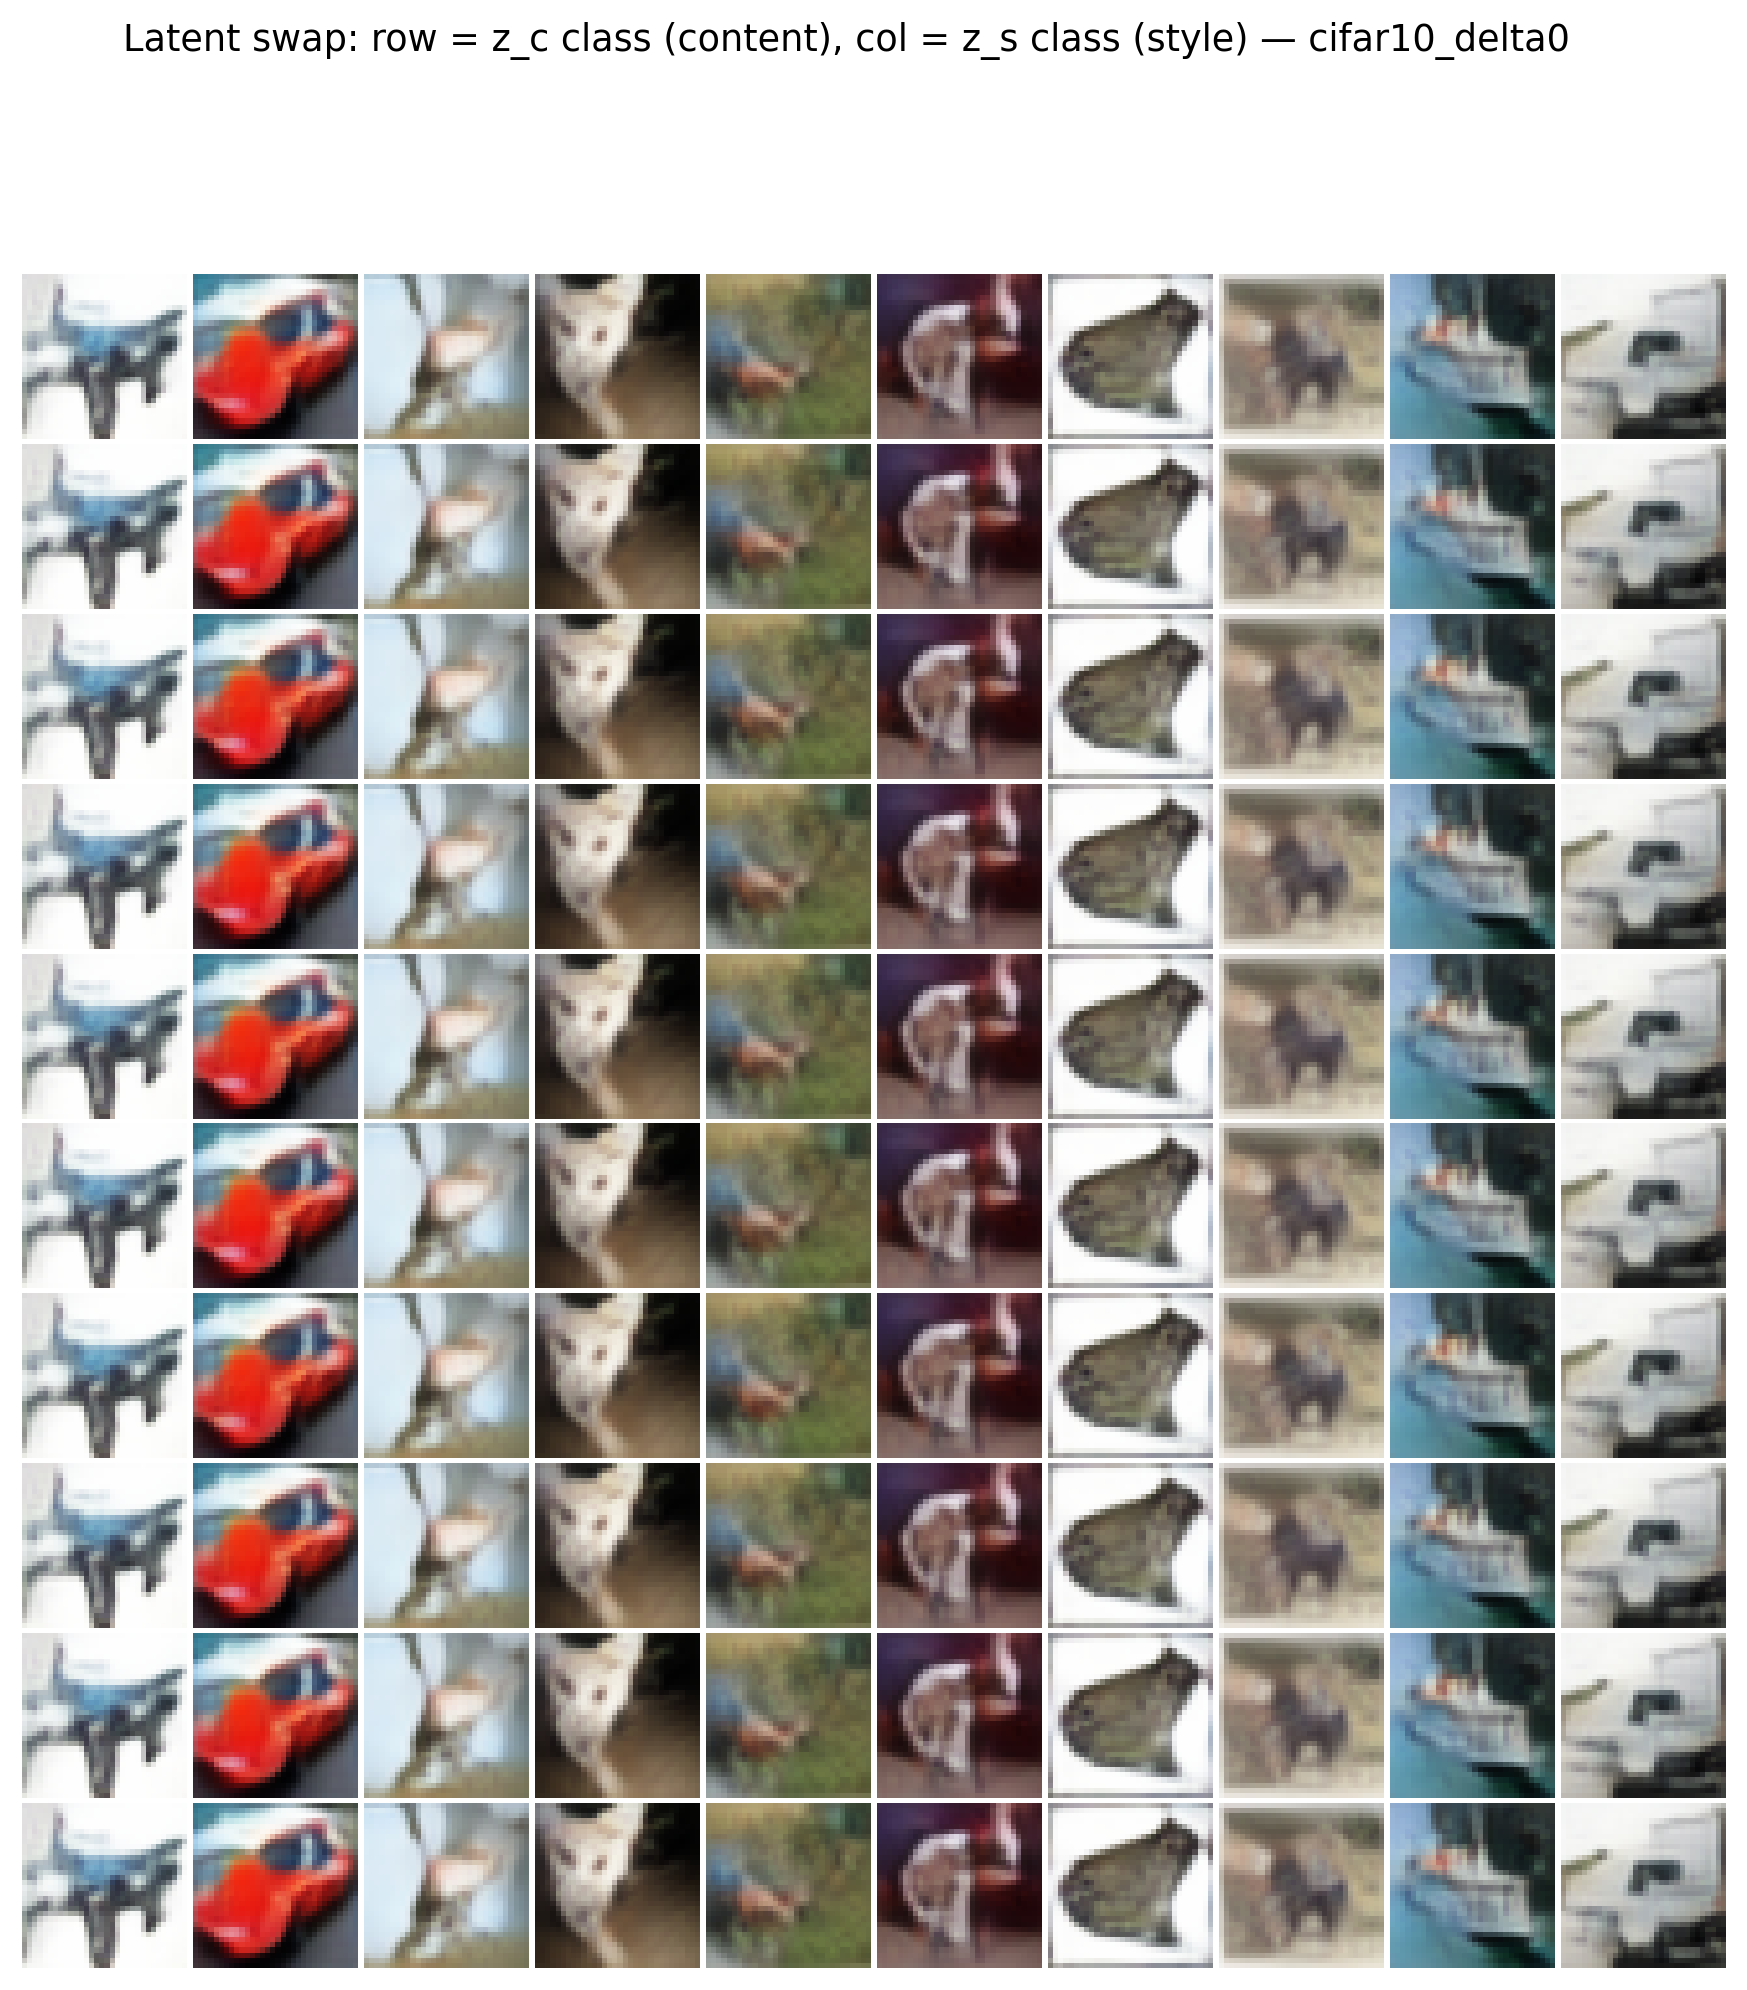
\includegraphics[width=0.86\linewidth]{cifar10_swap_grid_delta0.png}\\[-0.4em]
\small (b) CIFAR-10
\end{minipage}
\caption{Archived deterministic mean-swap grids at $\delta=0$.  Rows donate
semantic means and columns donate style means.  Column-controlled identity
is visually strong on MNIST and weaker but still present for several
CIFAR-10 classes.  Quantitative swap rates use the robustness-only internal
evaluator described above.}
\label{fig:swap-grid-app}
\end{figure}
\FloatBarrier

\section{Reproducibility and Current Evidence Boundary}
\label{app:reproducibility}

All Stage-0 results are stored as JSON plus SHA-256 sidecars.  Each manifest
records the repository state, checkpoint hash, evaluation seed, fixed subset,
latent view, probe split, feature preprocessing, and evaluator metadata.  The
canonical protocol version for the present draft is
\texttt{stage0-1.0.0}.  The five audited checkpoints are MNIST seed 0,
Fashion-MNIST seed 0, and CIFAR-10 seeds 0, 1, 2; all use evaluation seed 0.

The current draft intentionally excludes the earlier cross-model probe table,
multi-remedy comparison, five-seed remedy/sampling tables, and explicit
split-latent baseline ranges.  Those measurements were not yet regenerated
under the held-out Stage-0 protocol with complete artifacts.  They should be
reintroduced only after model-specific loaders, manifests, and canonical
outputs are available.  This boundary keeps every quantitative claim in the
present paper tied to an inspectable artifact.

The submission source, rendered author block, supplementary archive, and all
externally hosted materials must remain anonymous throughout review.


\end{document}
